 \documentclass{beamer}
%
% Choose how your presentation looks.
% For more themes, color themes and font themes, see:
% http://deic.uab.es/~iblanes/beamer_gallery/index_by_theme.html
%
\mode<presentation>
{
  \usetheme{Madrid}      % or try Darmstadt, Madrid, Warsaw, ...
  \usecolortheme{seahorse} % or try albatross, beaver, crane, ...
  \usefonttheme{serif}  % or try serif, structurebold, ...
  \setbeamertemplate{navigation symbols}{}
  \setbeamertemplate{caption}[numbered]
  \usepackage{amsmath}
  \usepackage{tcolorbox}
  \usepackage[export]{adjustbox}
  \tcbuselibrary{most}
  \usepackage{arydshln}
  \usepackage{tikz}
  \usetikzlibrary{plotmarks}
  \usepackage{pgfplots}
 %\usepackage{enumitem}
%\usepackage{enumerate}
  %\usepackage[shortlabels]{enumitem}
} 


\definecolor{myblue}{RGB}{65,105,225} 
\definecolor{myorange}{RGB}{250,190,0}

\setbeamercolor{structure}{fg=white,bg=myorange}
\setbeamercolor*{palette primary}{fg=myblue,bg=myorange}
\setbeamercolor*{palette secondary}{fg=white,bg=myblue}
\setbeamercolor*{palette tertiary}{bg=myblue,fg=white}
\setbeamercolor*{palette quaternary}{fg=white,bg=myorange!50}

\setbeamercolor{frametitle}{fg=black!90!myblue}

\setbeamercolor{section in head/foot}{fg=white,bg=myblue}
\setbeamercolor{author in head/foot}{fg=black,bg=myorange}
\setbeamercolor{title in head/foot}{fg=white,bg=myblue}

\setbeamertemplate{navigation symbols}{}

\setbeamertemplate{itemize/enumerate body begin}{\large}
\setbeamertemplate{itemize/enumerate subbody begin}{\large}


\defbeamertemplate*{headline}{mytheme}
{%
  \begin{beamercolorbox}[ht=2.25ex,dp=3.75ex]{section in head/foot}
    \insertnavigation{\paperwidth}
  \end{beamercolorbox}%
}%

\defbeamertemplate*{footline}{mytheme}
{
  \leavevmode%
  \hbox{%
  \begin{beamercolorbox}[wd=.5\paperwidth,ht=2.25ex,dp=1ex,right]{author in head/foot}%
    \usebeamerfont{author in head/foot}\insertshortauthor\hspace*{2em}
  \end{beamercolorbox}%
  \begin{beamercolorbox}[wd=.5\paperwidth,ht=2.25ex,dp=1ex,left]{title in head/foot}%
    \usebeamerfont{title in head/foot}\hspace*{2em}\insertshortsubtitle\hspace*{2em}
    \insertframenumber{} / \inserttotalframenumber
  \end{beamercolorbox}}%
  \vskip0pt%
}

\usepackage[english]{babel}
%\usepackage[utf8x]{inputenc}
\usepackage{xcolor}
\usepackage{listings}
\usepackage{pgf}  
\usepackage{textpos}
\usepackage{tabulary}
\usepackage{scrextend}
\usepackage{hyperref}
\usepackage{setspace}
\usepackage{rotating}
\lstset
{
    language=[LaTeX]TeX,
    breaklines=true,
    basicstyle=\tt\scriptsize,
    %commentstyle=\color{green}
    keywordstyle=\color{blue},
    %stringstyle=\color{black}
    identifierstyle=\color{magenta},
}
\newcommand{\bftt}[1]{\textbf{\texttt{#1}}}
%\newcommand{\comment}[1]{{\color[HTML]{008080}\textit{\textbf{\texttt{#1}}}}}
\newcommand{\cmd}[1]{{\color[HTML]{008000}\bftt{#1}}}
\newcommand{\bs}{\char`\\}
\newcommand{\cmdbs}[1]{\cmd{\bs#1}}
\newcommand{\lcb}{\char '173}
\newcommand{\rcb}{\char '175}
\newcommand{\cmdbegin}[1]{\cmdbs{begin\lcb}\bftt{#1}\cmd{\rcb}}
\newcommand{\cmdend}[1]{\cmdbs{end\lcb}\bftt{#1}\cmd{\rcb}}

\newcommand{\wllogo}{\textbf{Overleaf}}

% this is where the example source files are loaded from
% do not include a trailing slash
\newcommand{\fileuri}{https://raw.githubusercontent.com/GiancarloSucci/UniBo.IDSEPC.A2022/main/A2022.IDSEPCLaTeX/}


\usepackage{stackengine}
\def\Ruble{\stackengine{.67ex}{%
  \stackengine{.48ex}{\textsf{P}}{\rule{.8ex}{.12ex}\kern.6ex}{O}{r}{F}{F}{L}%
  }{\rule{.8ex}{.12ex}\kern.6ex}{O}{r}{F}{F}{L}\kern-.1ex}



%----------------------------------------------------------------------------------------
%	TITLE PAGE
%----------------------------------------------------------------------------------------
\title[L01]{Artificial Intelligence, Blockchain, e Criptovalute nello Sviluppo Software \newline\newline
Lezioni 8, 9, e 10: Fondamenti di Data Science per l'analisi dello sviluppo software} % The short title appears at the bottom of every slide, the full title is only on the title page

\author[{\tiny Giancarlo Succi }]{Giancarlo Succi\\\\ Dipartimento di Informatica -- Scienza e Ingegneria\\Universit\`{a} di Bologna\\
\bftt{g.succi@unibo.it}
} % Your name
\institute[unibo] % Your institution as it will appear on the bottom of every slide, may be shorthand to save space


\date{} % Date, can be changed to a custom date

\setbeamertemplate{navigation symbols}{}
\AtBeginSection[]
{
        \begin{frame}<beamer>{Outline}
                \tableofcontents[currentsection]
        \end{frame}
}
\begin{document}
\begin{frame}
\titlepage % Print the title page as the first slide

\end{frame}

%=============================================

\addtobeamertemplate{frametitle}{}{%
\begin{textblock*}{10mm}(-0.01mm,-0.95cm)

\includegraphics[width=0.9cm]{unibo-logo.png}
\end{textblock*}}

%=============================================

\begin{frame}
{\centerline{Struttura delle prime tre lezioni}}
\begin{itemize}
    \item Struttura del corso
    \item Il concetto di software
    \item Comprendere il problema
    \item La crisi del software
    \item Problemi \textit{Tame} e \textit{Wicked}
    \item Controllare il processo
    \item Meccanismi di coordinamento
    \item Modello di sviluppo a cascata
    \item Modello di sviluppo a spirale
    \item Il manifesto Agile
\end{itemize} 
\end{frame}

\begin{frame}
{\centerline{Struttura del corso}}
\begin{itemize}
    \item Si veda il sillabo alla pagina \url{https://github.com/GiancarloSucci/UniBo.AIBCCSS.P2023/blob/main/P2023.AIBCCSS.Sillabo.pdf}
\end{itemize} 
\end{frame}


\begin{frame}
{\centerline{Il concetto di software}}
\begin{itemize}
    \item La natura del software
    \item La funzione di costo
    \item Il software come economia di rete 
    \item Competizione nel mercato software
\end{itemize} 
\end{frame}

\begin{frame}
{\centerline{La natura del software (1/3)}}
\begin{itemize}
    \item Il software \`{e} il risultato di un atto creativo della mente umana
\end{itemize} 
\vspace{0.8cm}
\begin{center}
    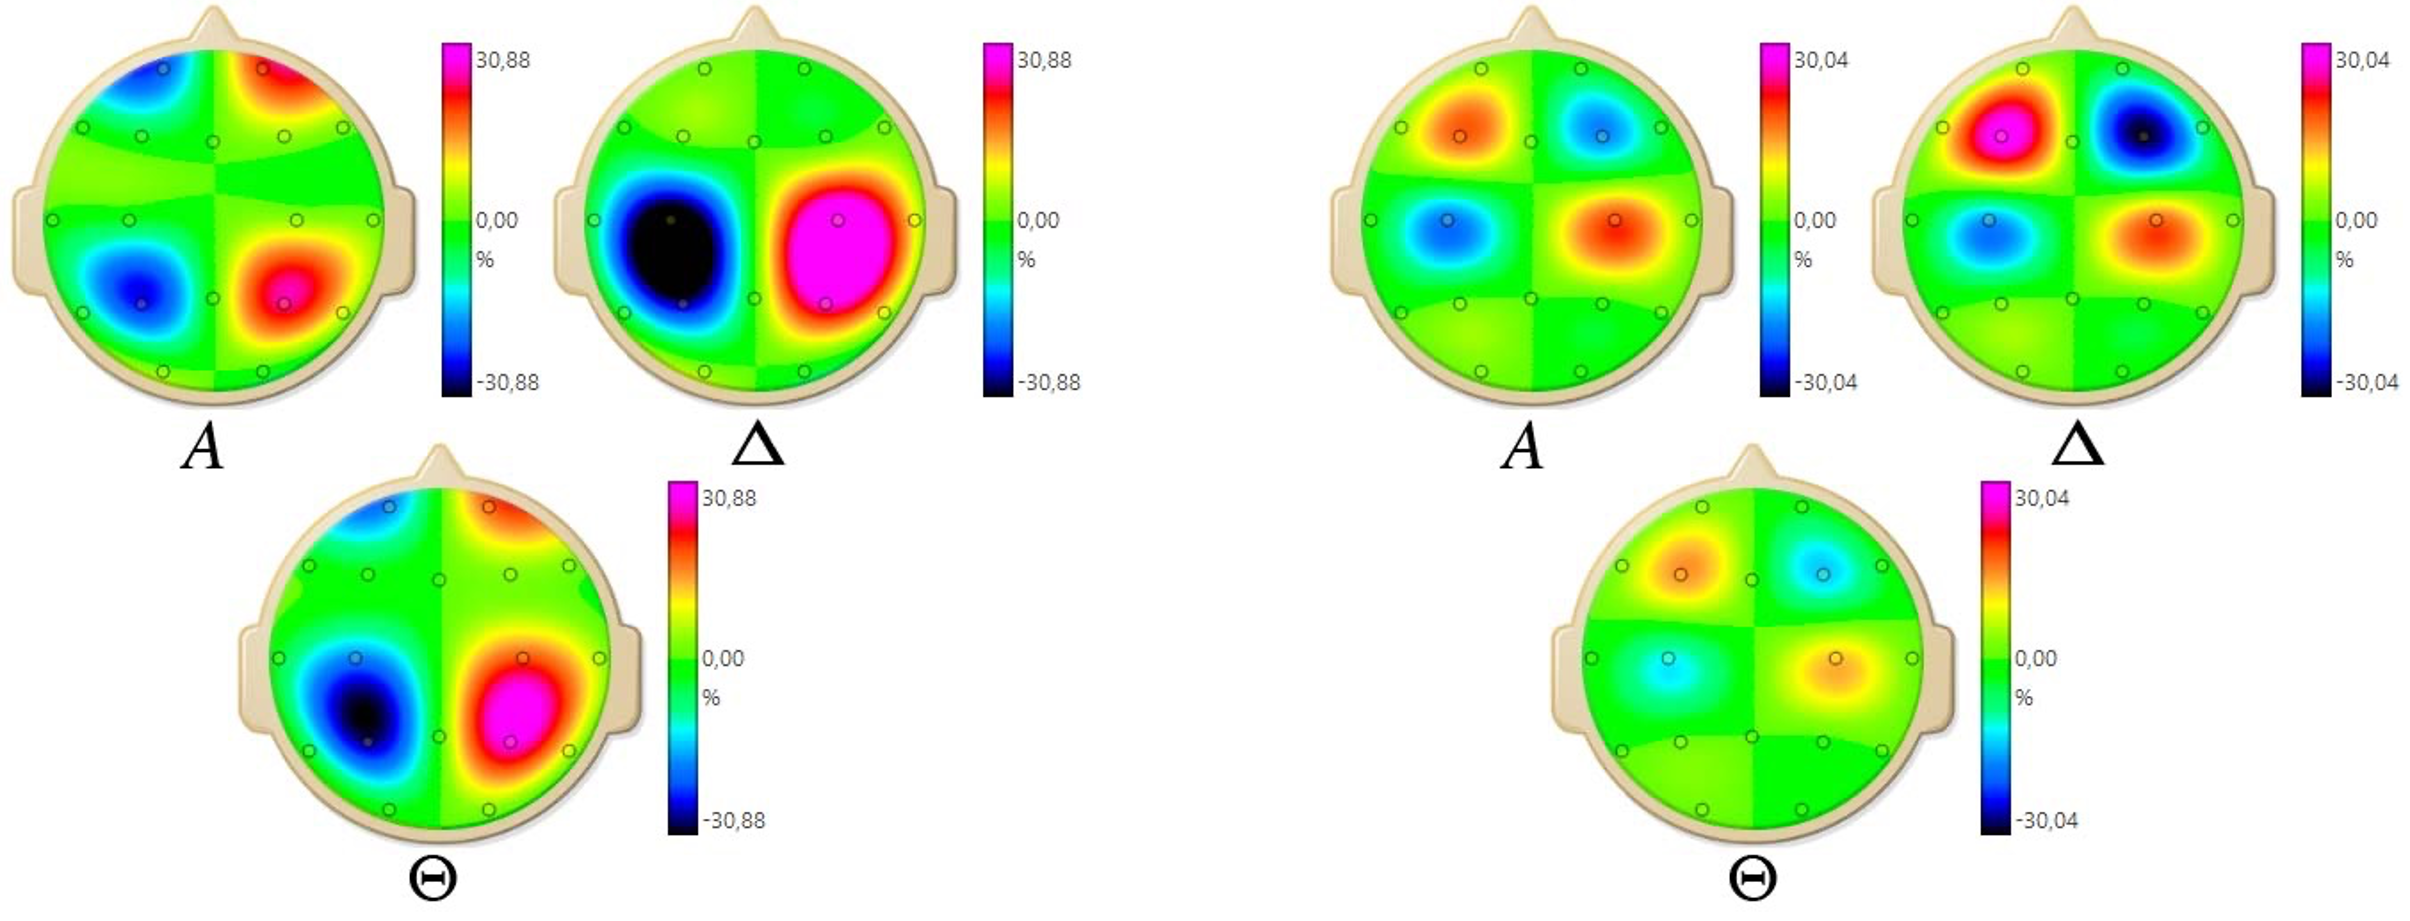
\includegraphics[width=\textwidth]{P2023.AIBCCSS.IlConcettoDiSoftware/SoftwareAttoCreativoEEG.png}
\end{center}

\end{frame}

\begin{frame}
{\centerline{La natura del software (2/3)}}
\begin{itemize}
    \item Il software \`{e} simile ad altri risultati di creazioni umane
\end{itemize} 
\begin{center}
    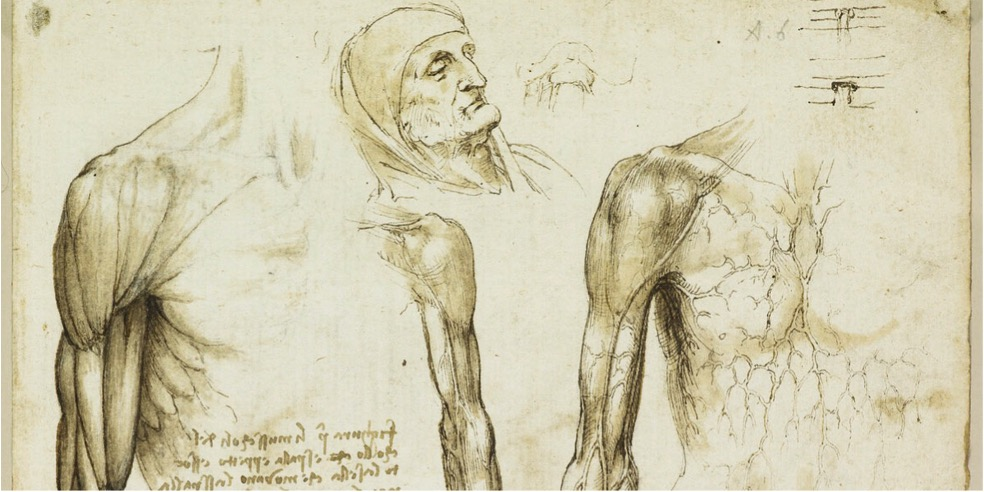
\includegraphics[width=\textwidth]{P2023.AIBCCSS.IlConcettoDiSoftware/SoftwareAttoCreativoLeonardo.jpg}
\end{center}

\end{frame}

\begin{frame}
{\centerline{La natura del software (3/3)}}
\begin{itemize}
    \item Il software \`{e} protetto dal diritto d'autore (anche se la questione \`{e} sempre aperta)
\begin{itemize}
    \item I diritti degli sviluppatori sono divisi in diritti morali (non alienabili) e diritti economici (alienabili)
    \item I diritti dei creatori sono protetti anche se non registrano un brevetto 
    \item I diritti durano molto pi\`{u} a lungo di quelli di un brevetto -- 50 anni dopo la morte del creatore invece che 20 anni dopo la registrazione del brevetto 
    \item Il software \`{e} dato in licenza e non venduto
\end{itemize} 
\end{itemize} 

\end{frame}

\begin{frame}
{\centerline{La funzione di costo}}
\begin{center}
    \begin{tikzpicture}[scale=0.9]
\begin{axis}[
axis x line=center,
axis y line=center,
xmin = -0.95,
xmax = 9.95,
ymin = -0.95,
ymax = 11,
title={Costo marginale per unit\`{a}},
xlabel = {Numero di unit\`{a} prodotte},
yticklabels={,,},
extra x ticks = {0},
extra x tick label = {$\hspace{-0.6cm}0$},
]
\addplot[very thick,domain=0.01:0.94,samples=100,red] {0.040*x/(ln(x)^2)};
\addplot[very thick,domain=0.94:1.06,samples=10,red] {0.040*0.94/(ln(0.94)^2)};
\addplot[very thick,domain=1.06:10,samples=100,red] {0.032*x/(ln(x)^2});
\addplot[very thick,dotted] coordinates {(1,0) (1,10)};
\addplot[thick,dashed,green] coordinates {(0,10) (10,10)};
\end{axis}
\end{tikzpicture}
\end{center}

\end{frame}

\begin{frame}
{\centerline{Esercizio proposto}}
\vspace{1cm}
\begin{center}
    \LARGE{Trovare altri settori in cui si notano funzioni di costo simili.}
\end{center}

\end{frame}


\begin{frame}
{\centerline{La segmentazione del mercato nel software}}
\begin{itemize}
\item Nel software non ci sono limiti fisici alla segmentazione
\item Inoltre:
\begin{itemize}
\item il software \`{e} protetto dal copyright
\item la funzione di costo ha una struttura a ``L''
\end{itemize}
\item Si pu\`{o} quindi operare un segmentazione aggressiva
\item Si possono operare strategie di ``bundling'' per promuovere nuovi prodotti
\end{itemize}

\end{frame}

\begin{frame}
{\centerline{Esempio di segmenti di mercato}}

\begin{itemize}
    \item Questi dati sono molto vecchi, ma il succo non cambia:
\end{itemize}

\begin{center}
    
\resizebox{0.9\textwidth}{!}{%
  \begin{tabular}{|c|c|c|c|}
  \hline
  \textbf{Prodotto} & \textbf{Professional} & \textbf{Educational} & \textbf{E/P} \\
  \hline
    Office 97 & \$ 779 & \$ 215.45 & 27.6\% \\ \hline
    Corel WP Suite 98 & \$ 449 & \$ 71.55 & 15.9\% \\
  \hline
  \end{tabular}

} % end of scope of "\resizebox"  directive
\end{center}
\end{frame}

\begin{frame}
{\centerline{Altro esempio di segmentazione (16/09/2022)}}
\begin{center}
    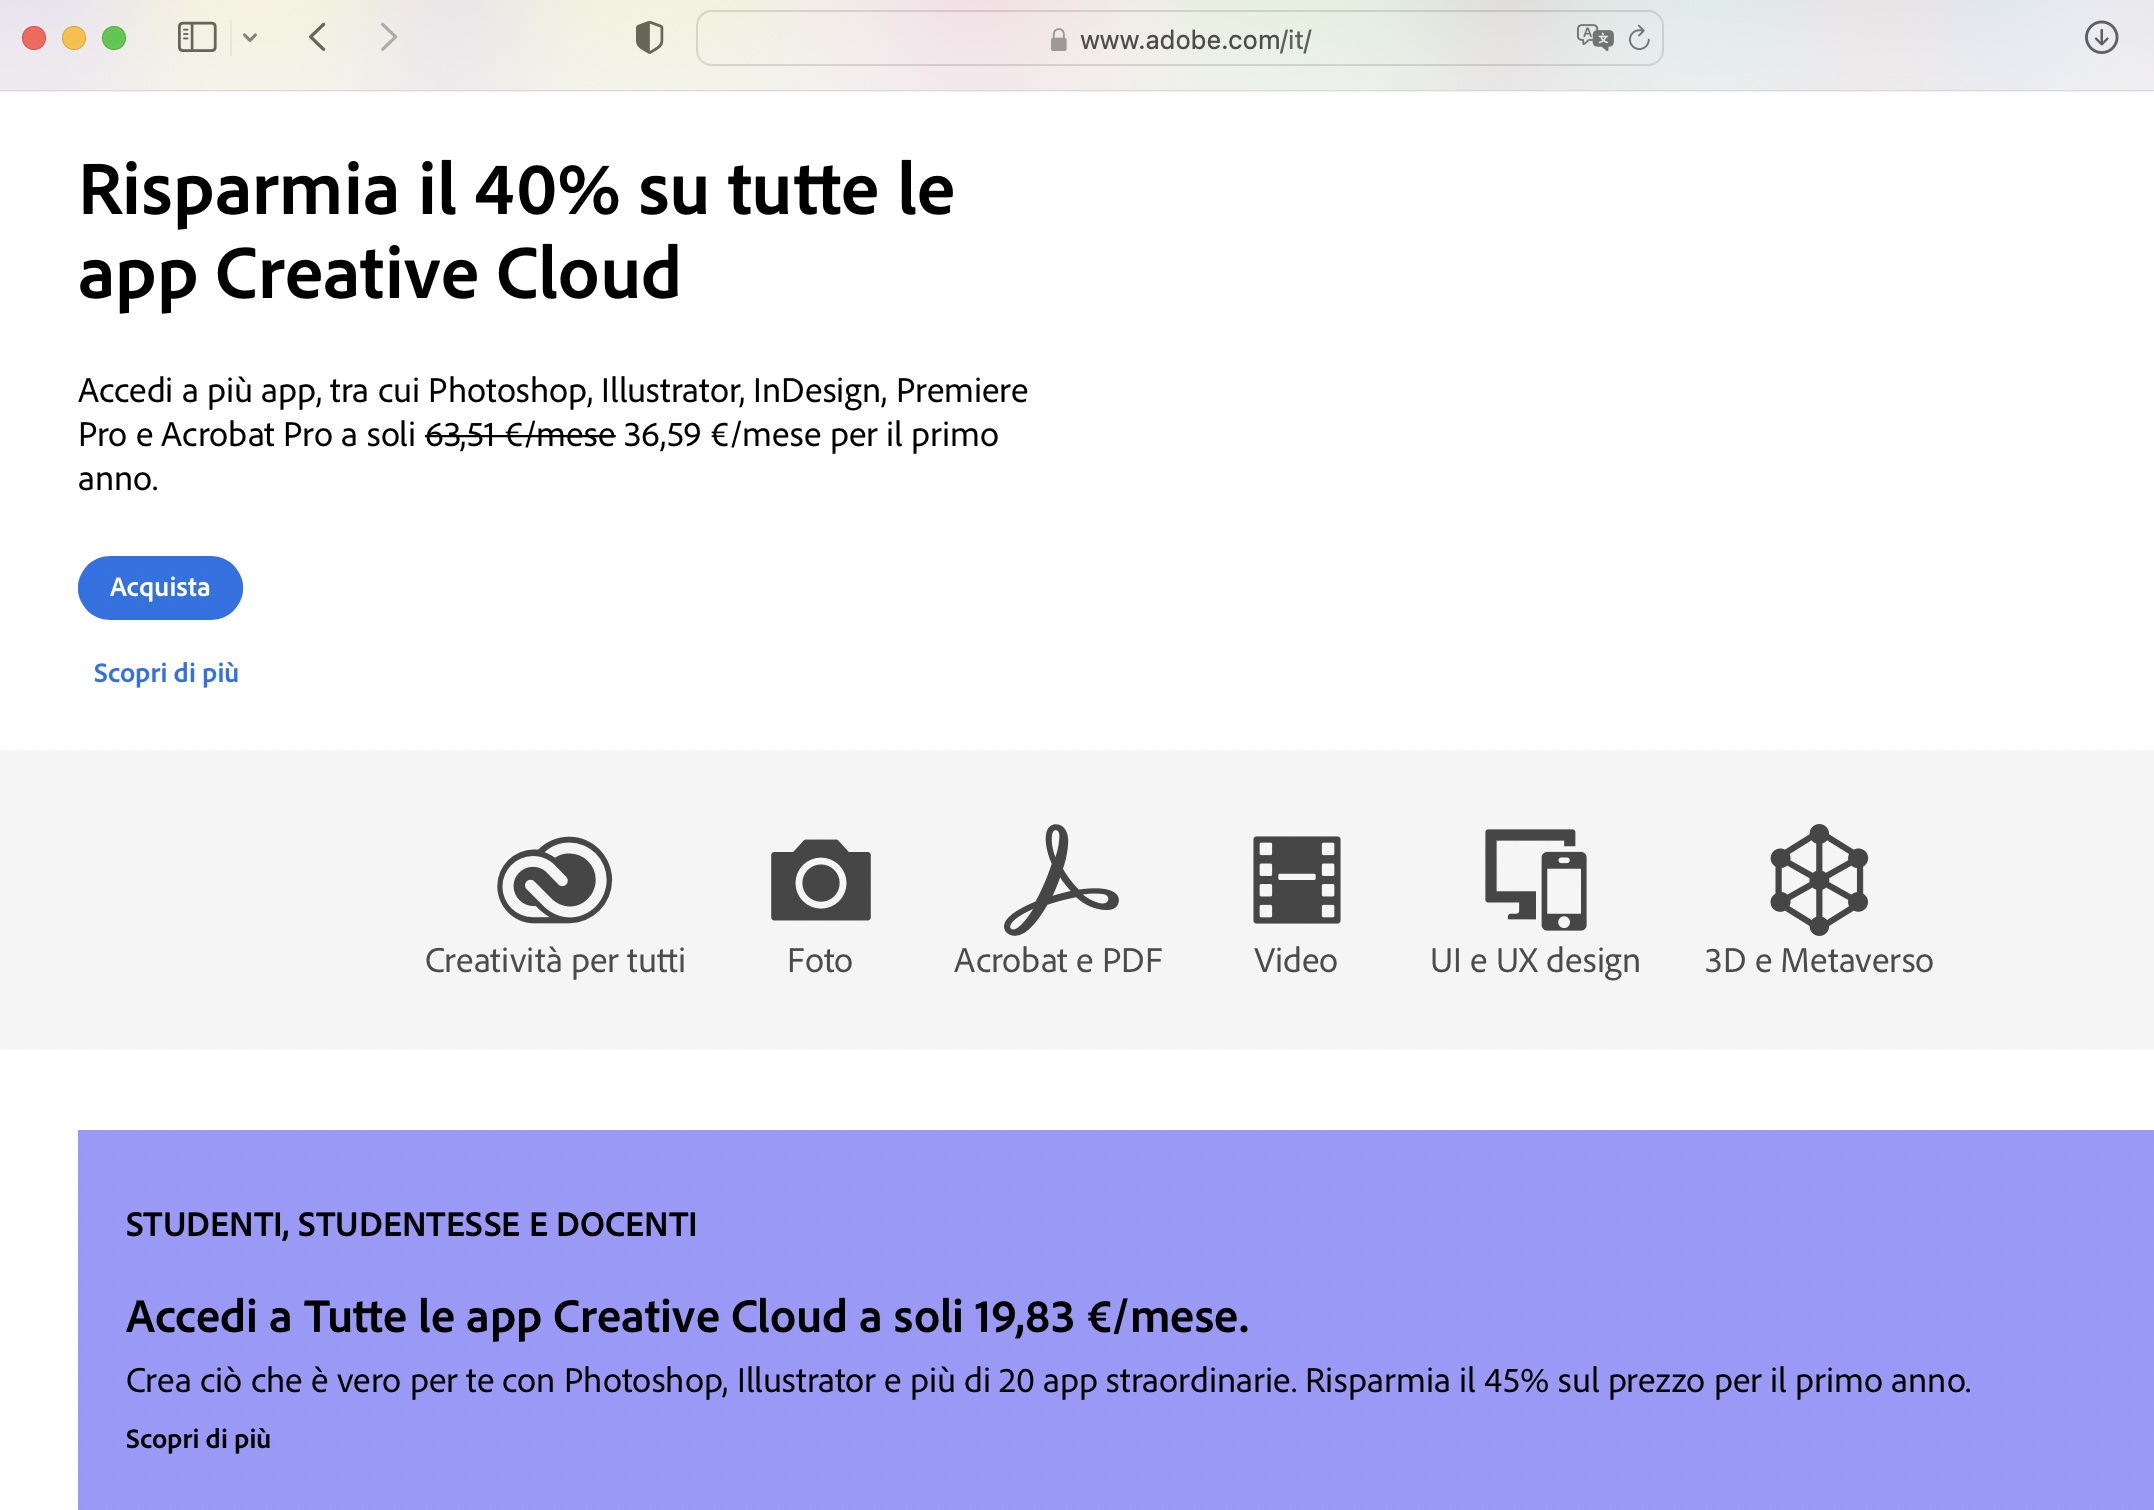
\includegraphics[width=0.8\textwidth]{P2023.AIBCCSS.IlConcettoDiSoftware/SegmentationBundlingAdobe.jpg}
\end{center}

\end{frame}

\begin{frame}
{\centerline{Bundling (16/09/2022)}}
\begin{center}
    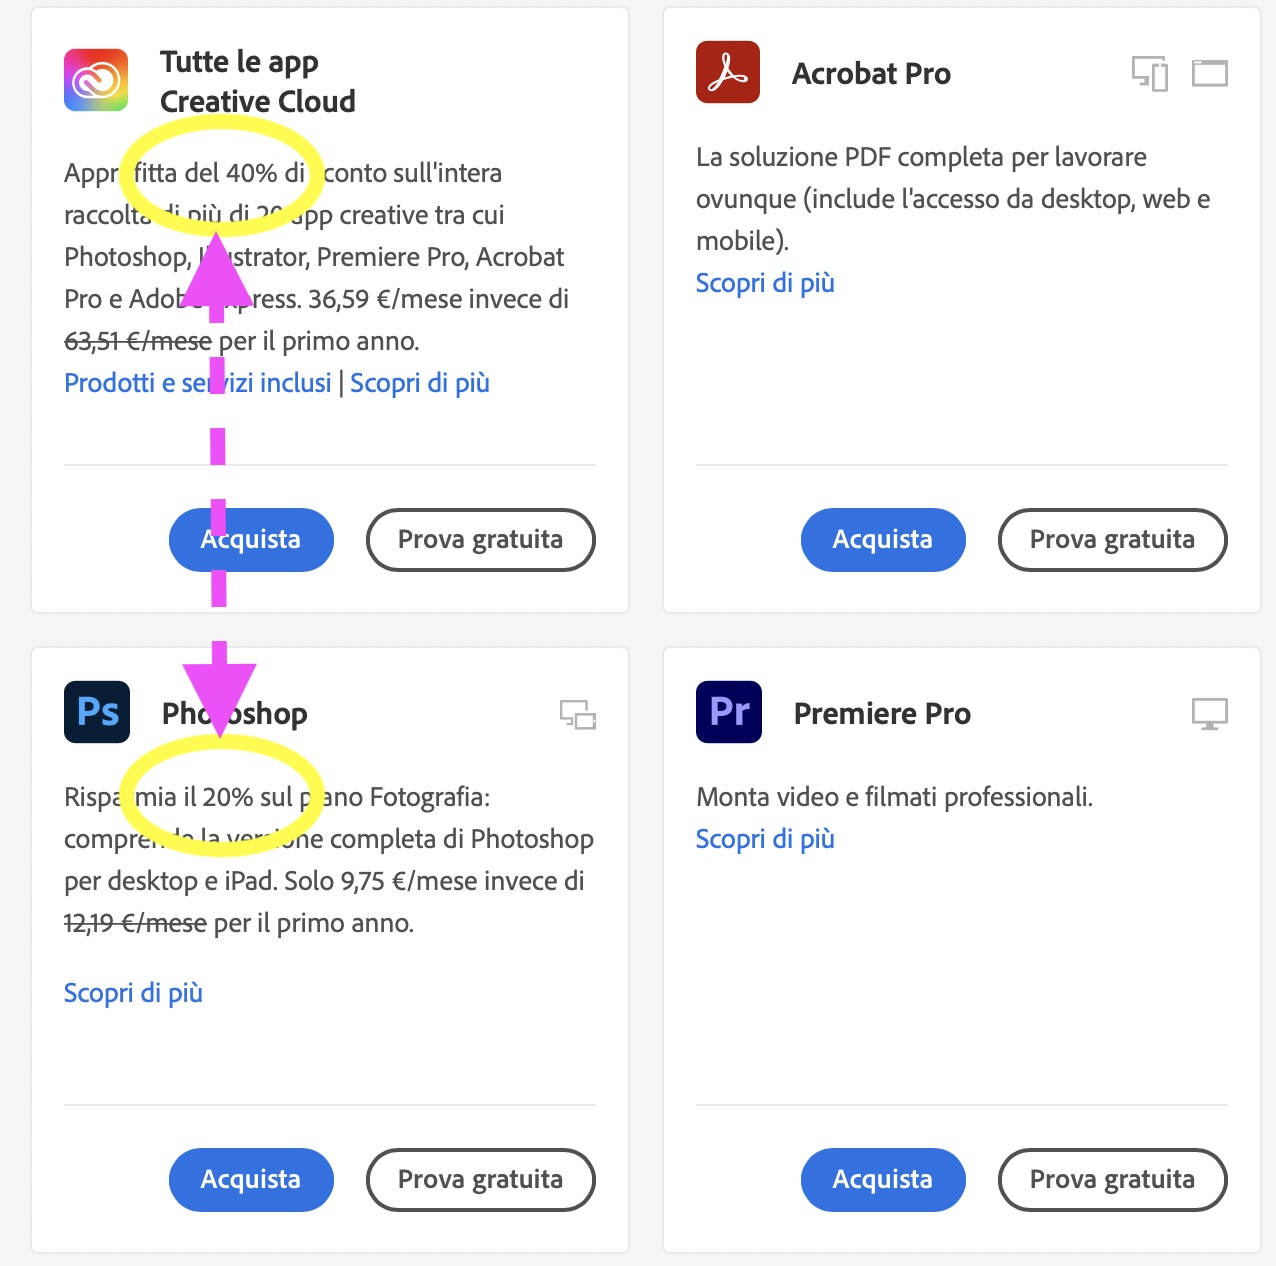
\includegraphics[width=0.6\textwidth]{P2023.AIBCCSS.IlConcettoDiSoftware/BundlingAdobe.jpg}
\end{center}

\end{frame}

\begin{frame}
{\centerline{Bundling in altri settori ``creativi'' (1/2)}}
\begin{center}
    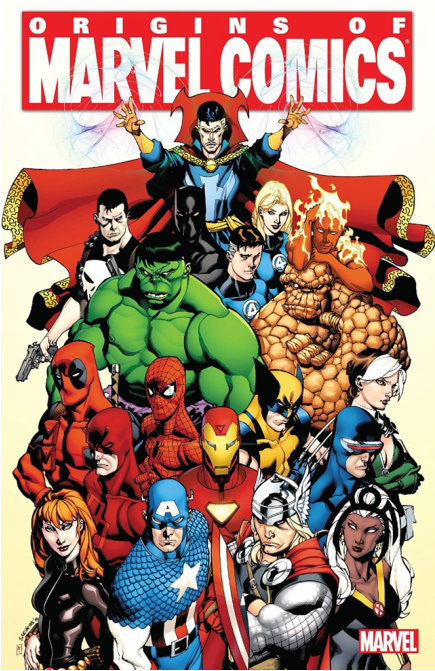
\includegraphics[width=0.4\textwidth]{P2023.AIBCCSS.IlConcettoDiSoftware/BundlingMarvel.pdf}
\end{center}

\end{frame}

\begin{frame}
{\centerline{Bundling in altri settori ``creativi'' (2/2)}}
\begin{center}
    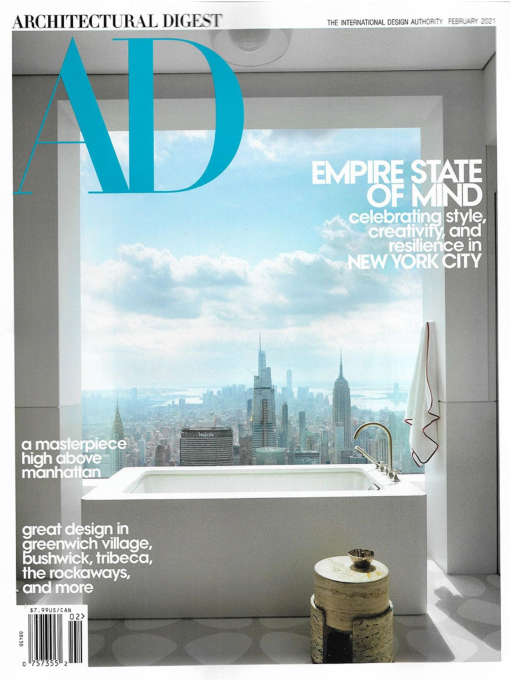
\includegraphics[width=0.45\textwidth]{P2023.AIBCCSS.IlConcettoDiSoftware/BundlingAD.pdf}
\end{center}

\end{frame}

\begin{frame}
{\centerline{Esercizio proposto}}
\vspace{1cm}
\begin{center}
    \LARGE{Presentare esempi di bundling sperimentati di persona.}
\end{center}

\end{frame}



\begin{frame}
{\centerline{Esternalit\`{a} di rete}}

\begin{itemize}
\item Si hanno \textcolor{blue}{economie di rete} per un prodotto quando un utente lo valuta  diversamente se ci sono utenti di tale prodotto o di prodotti \textit{compatibili}.

\item Quando il valore di un prodotto aumenta quanti pi\`{u} ci sono utenti di tale prodotto o di prodotti compatibili si dice che ci sono \textcolor{red}{esternalit\`{a} di rete}, o, semplicemente \textcolor{red}{esternalit\`{a}}.


\end{itemize}

\end{frame}

\begin{frame}
{\centerline{Esempi di esternalit\`{a} di rete}}

\begin{itemize}
\item Il mercato delle telecomunicazioni \`{e} un chiaro esempio di esternalit\`{a} di rete: 
\begin{itemize}
\item il valore di un telefono dipende da quanti utenti lo usano. Se nessuno lo usasse, sarebbe inutile!
\end{itemize}
\item Anche il mercato delle figurine Panini \`{e} un chiaro esempio di esternalit\`{a} di rete!

\item Non tutti i mercati hanno esternalit\`{a} di rete: quello delle automobili di lusso, sicuramente no:
\begin{itemize}
\item chi compera un'auto di lusso spera probilmente di essere l'unico nel suo circolo ad averla.
\end{itemize}
\item La stessa situazione si ha con i vestiti di lusso.

\end{itemize}

\end{frame}

\begin{frame}
{\centerline{Esternalit\`{a} di rete nel software}}

\begin{itemize}
\item L'industria software ha forti esternalit\`{a} di rete.
\item Ci sono due chiari esempi di tali esternalit\`{a}:
\begin{itemize}
\item lo scambio di informazioni, ad esempio via posta elettronica o tramite la condivisione di formati di file (ad esempio .docx o .odt)
\item l'usabilit\`{a} dei sistemi software, per cui se si conosce la modalit\`{a} di uso di un sistema, si tende ad usare sistemi con le stesse modalit\`{a}, ad esempio, con le stesse scorciatoie
\end{itemize}

\end{itemize}

\end{frame}

\begin{frame}
{\centerline{Esercizio proposto}}
\vspace{1cm}
\begin{center}
    \LARGE{Identificare casi di esternalit\`{a} di rete presenti nella vita di ogni giorno.}
\end{center}

\end{frame}


\begin{frame}
{\centerline{Effetti delle esternalit\`{a} di rete (1/3)}}

\begin{itemize}
\item I mercati con forti esternalit\`{a} di rete stimolano le aziende a saltare sul carro di nuove tecnologie, anche se tali tecnologie devono ancora provare la loro efficacia;
\begin{itemize}
\item questo fenomeno viene chiamato \textcolor{red}{insufficient friction} (frizione insufficiente) oppure \textcolor{blue}{excess bandwagon} (carrozzone eccessivo).
\end{itemize}

\end{itemize}

\end{frame}

\begin{frame}
{\centerline{Effetti delle esternalit\`{a} di rete (2/3)}}

\begin{itemize}
\item Le esternalit\`{a} possono produrre effetti di riduzione della fluidit\`{a} degli uteni su prodotti
\begin{itemize}
\item ci\`{o} viene chiamato \textcolor{red}{lock-in} (chiusura) e si manifesta con la presenza di \textcolor{blue}{barriere di ingresso}, ovvero la necessit\`{a} di costi aggiuntivi per passare ad altri prodotti equivalenti o equivalenti a prodotti compatibili
\end{itemize}
\item Un tipico esempio di questo è stato il formato Betamax \url{https://it.wikipedia.org/wiki/Betamax}

\end{itemize}

\end{frame}


\begin{frame}
{\centerline{Effetti delle esternalit\`{a} di rete (3/3)}}

\begin{itemize}

\item La presenza di un monopolista in un mercato ad alta tecnologia con esternalit\`{a} di rete pu\`{o} incutere paura a possibili compratori timorosi di affidarsi ad un singolo venditore in quanto:
\begin{itemize}
\item agli occhi dei potenziali compratori il mercato pu\`{o} essere considerato ancora troppo immaturo,
\item i potenziali compratori possono aver paura che il monopolista collassi o aumenti arbitrariamente i prezzi dei prodotti.
\end{itemize}

\end{itemize}

\end{frame}


\begin{frame}
{\centerline{Esercizio proposto}}
\vspace{1cm}
\begin{center}
    \LARGE{Trovare effetti delle tre esternalit\`{a} di rete nella propria esperienza.}
\end{center}

\end{frame}

\begin{frame}
{\centerline{Visualizzazione del mercato -- Valore}}
\begin{itemize}
    \item Come analizzare il valore del prodotto
\end{itemize} 
\begin{center}
    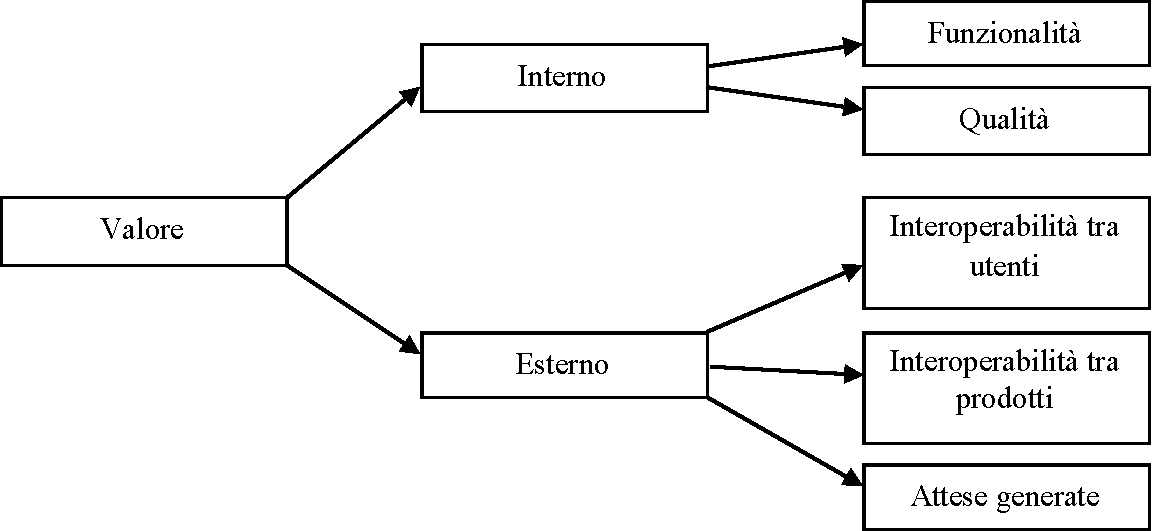
\includegraphics[width=\textwidth]{P2023.AIBCCSS.IlConcettoDiSoftware/ValoreDelProdotto.pdf}
\end{center}

\end{frame}

\begin{frame}
{\centerline{Visualizzazione del mercato -- Compatibilit\`{a}}}
\begin{itemize}
    \item Come analizzare la compatibilit\`{a} tra prodotti via formati dei dati
\end{itemize} 
\begin{center}
    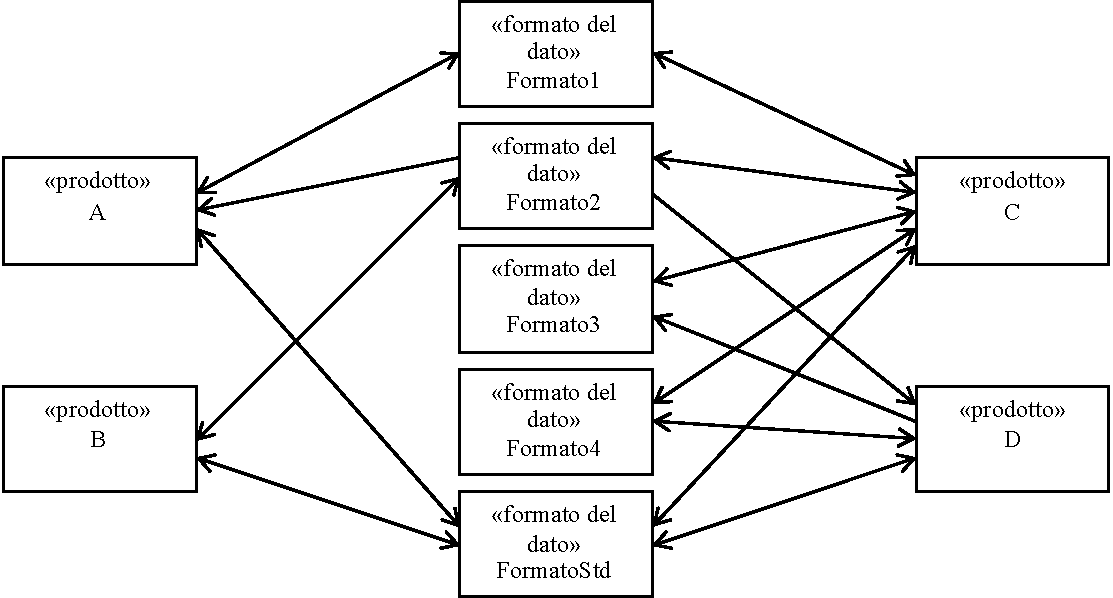
\includegraphics[width=0.9\textwidth]{P2023.AIBCCSS.IlConcettoDiSoftware/CompatibilitaProdotti.pdf}
\end{center}

\end{frame}
\begin{frame}
{\centerline{Esempi di compatibilit\`{a} (1/2)}}
\begin{itemize}
    \item Esempio di come presentare le compatibilit\`{a} per Word
\end{itemize} 
\begin{center}
    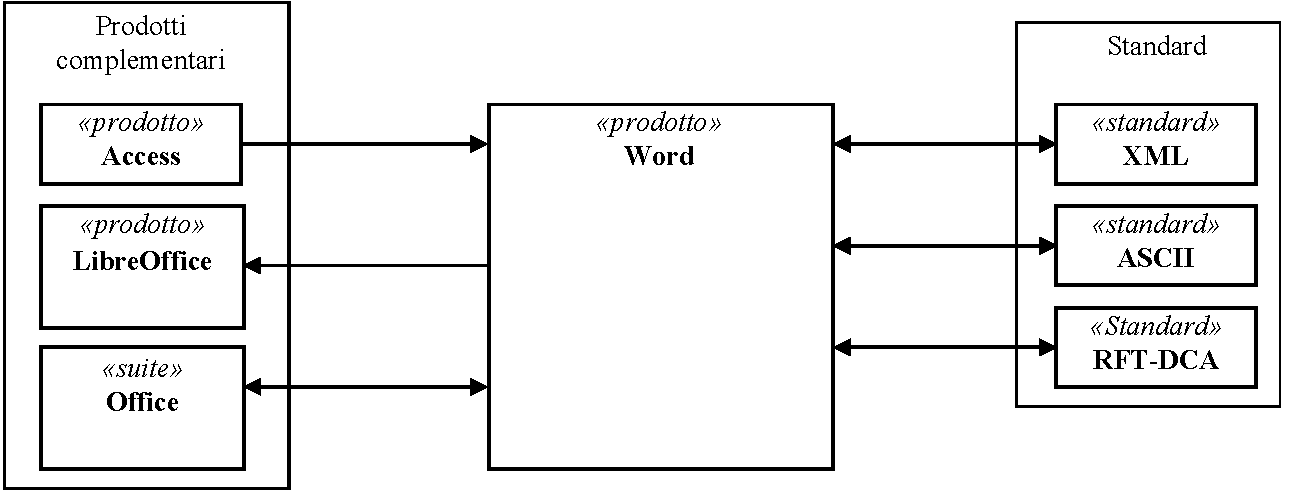
\includegraphics[width=0.9\textwidth]{P2023.AIBCCSS.IlConcettoDiSoftware/EsempiCompatibilita.1.pdf}
\end{center}

\end{frame}

\begin{frame}
{\centerline{Esempi di compatibilit\`{a} (2/2)}}
\begin{itemize}
    \item Esempio di come presentare le compatibilit\`{a} per Word
\end{itemize} 
\begin{center}
    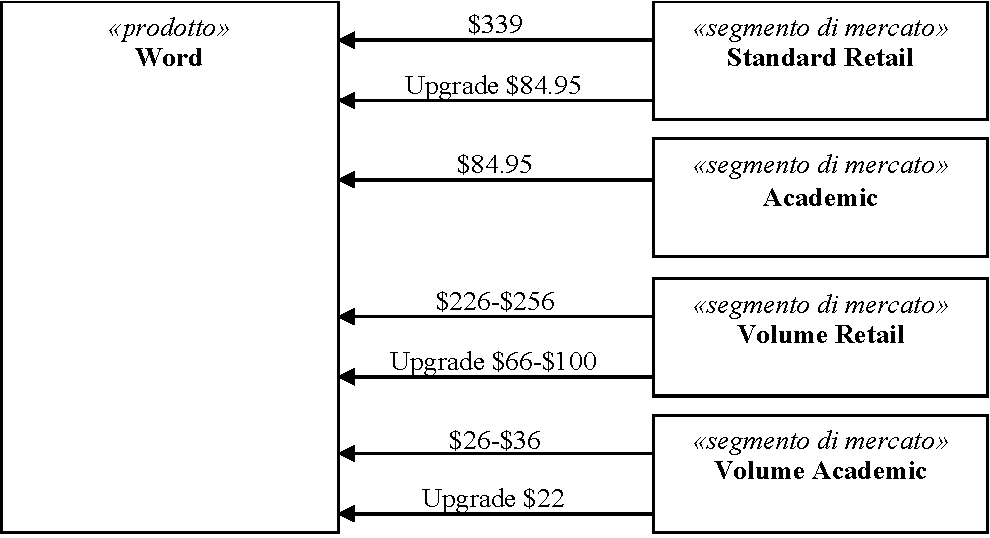
\includegraphics[width=0.9\textwidth]{P2023.AIBCCSS.IlConcettoDiSoftware/EsempiCompatibilita.2.pdf}
\end{center}

\end{frame}

\begin{frame}
{\centerline{Esercizio proposto}}
\vspace{1cm}
\begin{center}
    \LARGE{Tracciare il diagramma di compatibilit\`{a} per un prodotto soggetto a esternalit\`{a} a vostra scelta.}
\end{center}

\end{frame}


\begin{frame}
{\centerline{Strategie comunemente utilizzate}}

\begin{itemize}
    \item Upgrade di prodotti
    \item Upgrade competitivi
    \item Suite di prodotti
\end{itemize}

\vspace{1cm}
\begin{center}
    
\resizebox{0.9\textwidth}{!}{%
  \begin{tabular}{|c|c|c|c|}
  \hline
  \textbf{Strategia} & \textbf{Esternalit\`{a}} & \textbf{Bundling} & \textbf{Segmentazione} \\
  \hline
    Upgrade di prodotti & $\times$ &  -- & $\times$ \\ \hline
    Upgrade competitivi & $\times$ & -- & $\times$ \\ \hline
    Suite di prodotti & $\times$ & $\times$ & -- \\
  \hline
  \end{tabular}

} % end of scope of "\resizebox"  directive
\end{center}

\end{frame}

\begin{frame}
{\centerline{Esercizio proposto}}
\vspace{1cm}
\begin{center}
    \LARGE{Identificare strategie presenti nel prodotto soggetto a esternalit\`{a} da voi precedentemente prescelto.}
\end{center}

\end{frame}

\begin{frame}
{\centerline{Indice}}
\begin{itemize}
    \item Comprendere il problema
    \item La crisi del software
    \item Problemi \textit{Tame} e \textit{Wicked}
    \item Controllare il processo
    \item Meccanismi di coordinamento
    \item Modello di sviluppo a cascata
    \item Modello di sviluppo a spirale
    \item Il manifesto Agile
\end{itemize} 
\end{frame}

\begin{frame}{\centerline{Comprendere il problema}}

\begin{center}
{\Large
Ariane 5 (1996)\\
}
\end{center}
\begin{center}
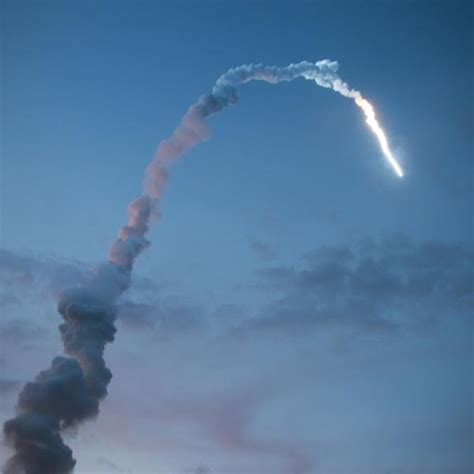
\includegraphics[width=60mm]{P2023.AIBCCSS.IlConcettoDiSoftware/Ariane5.jpeg}
\end{center}

\end{frame}



\begin{frame}{\centerline{Software Engineering (1/2)}}

\begin{center}
Software Engineering o Ingegneria del Software\\
\vspace{1cm}
{\Large
Ingegnerizzare la produzione del software\\
}
\vspace{2cm}
Spesso si fanno analogie tra la produzione del software e cucinare...
\end{center}
\end{frame}

\begin{frame}{\centerline{Software Engineering (2/2)}}

\begin{center}
\Large
Che lo show abbia inizio!\\
\vspace*{0.5cm}
Signore e signori: \textcolor{red}{Charlie Chaplin}
\end{center}
\begin{center}
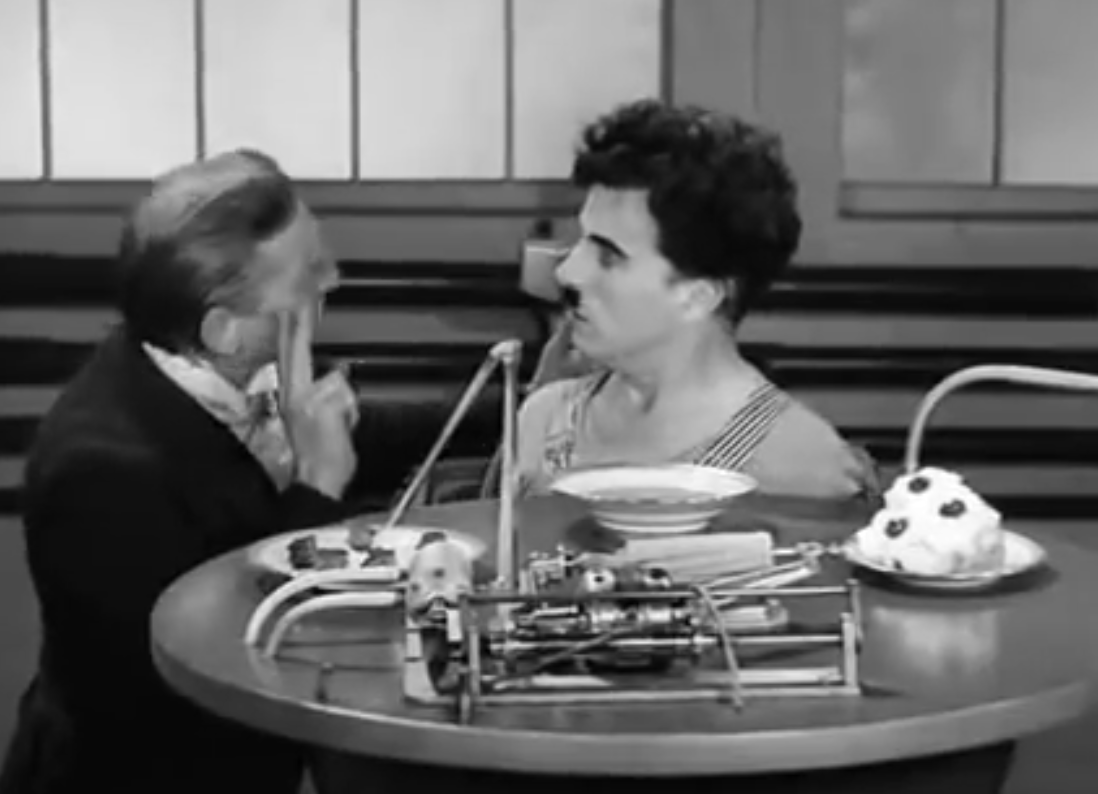
\includegraphics[width=60mm]{P2023.AIBCCSS.IlConcettoDiSoftware/Chaplin_ModernTimes.png}
\end{center}

\end{frame}



\begin{frame}{\centerline{Sondaggio}}
\begin{center}
Sulla base del video, qual \`{e} lo scopo dell'ingegneria dle software?
\end{center}
\end{frame}

\begin{frame}{\centerline{Idee}}
\noindent\makebox[\linewidth]{\rule{\paperwidth}{0.4pt}}\\
\vspace{0.5cm}

\noindent\makebox[\linewidth]{\rule{\paperwidth}{0.4pt}}\\
\vspace{0.5cm}

\noindent\makebox[\linewidth]{\rule{\paperwidth}{0.4pt}}\\
\vspace{0.5cm}

\noindent\makebox[\linewidth]{\rule{\paperwidth}{0.4pt}}\\
\vspace{0.5cm}

\noindent\makebox[\linewidth]{\rule{\paperwidth}{0.4pt}}\\
\vspace{0.5cm}

\noindent\makebox[\linewidth]{\rule{\paperwidth}{0.4pt}}\\
\vspace{0.5cm}

\noindent\makebox[\linewidth]{\rule{\paperwidth}{0.4pt}}\\

\end{frame}

\begin{frame}{\centerline{La mia idea dell'ingegnere del software}}

\begin{center}
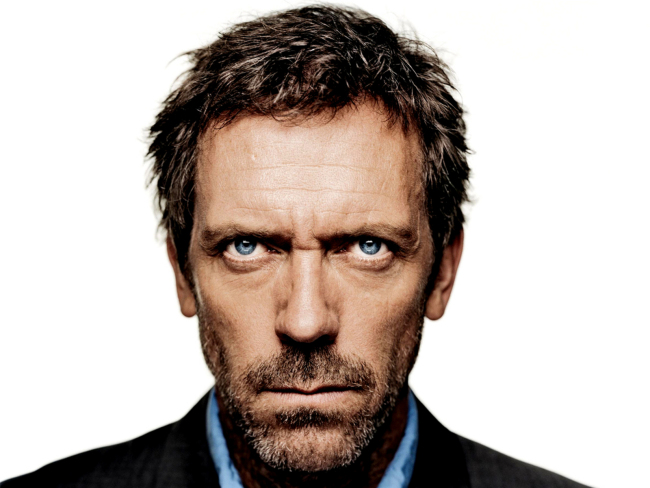
\includegraphics[width=80mm]{P2023.AIBCCSS.IlConcettoDiSoftware/DrHouse_SoftwareEngineer.jpg}
\end{center}

\end{frame}

\begin{frame}{\centerline{Continuiamo lo show!}}
\vspace*{1.5cm}
\begin{center}
\Huge Video on Dr. House

\end{center}

\end{frame}

\begin{frame}{\centerline{Lean Software Development}}
Lean software development o approccio lean alla produzione del software\\
\vspace{1cm}
\begin{center}
Lean software development o approccio lean alla produzione del software\\
\vspace{1cm}
\LARGE
Premesse sul Lean Management
\end{center}
\end{frame}

\begin{frame}{\centerline{La ``Software Crisis'' (1/3)}}

La ``Software Crisis'' o ``crisi del software'' \`{e} il fenomeno dovuto all'aumento della potenza dei calcolatori: in termini \textit{terra terra}, finch\'{e} i calcolatori erano molto piccoli, la programmazione non presentava problemi, quando le macchine hanno iniziate a crescere, i problemi hanno iniziato a comparire, e ora che abbiamo computer giganteschi, la programmazione è pure diventata un problema gigantesco.\\
Edsger Dijkstra, \textcolor{red}{\bf 1972}
\begin{center}
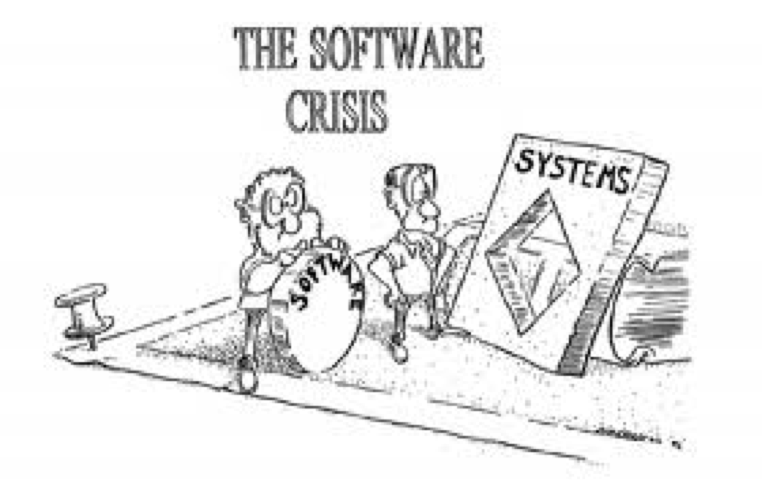
\includegraphics[width=55mm]{P2023.AIBCCSS.IlConcettoDiSoftware/pic-01.png}
\end{center}



\begin{center}
\tiny
\url{http://qualityandprogramming.blogspot.ru/2012/03/crisis-del-software.html}
\end{center}

\end{frame}

\begin{frame}{\centerline{La ``Software Crisis'' (2/3)}}

Sequenze di rivoluzioni tecnologiche si sono viste in molte aree dello scibile umano grazie al software.

\begin{center}
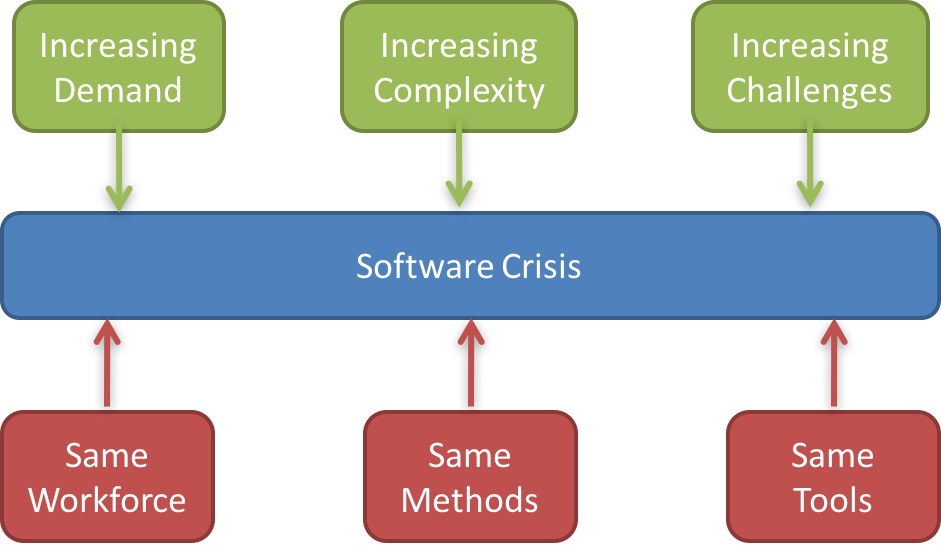
\includegraphics[width=80mm]{P2023.AIBCCSS.IlConcettoDiSoftware/pic-02.png}
\end{center}
Purtroppo, l'ingegneria del software non ha avuto una analoga rivoluzione!

\begin{center}
\tiny
\url{http://www.slideshare.net/rui\_curado/abse-and-atomweaver-a-quantum-leap-in-software-development}
\end{center}



\end{frame}
\begin{frame}{\centerline{La ``Software Crisis'' (3/3)}}

Le cause della crisi del software sono collegate  alla complessit\`{a} crescente di hardware e software associato, e tale crisi si \`{e} manifestata in una moltitudine di modi:
\begin{itemize}
\item Progetti che sforano il budget
\item Progetti che non rispettano i tempi
\item Sistemi software inefficienti
\item Sistemi software di bassa qualit\`{a}
\item Sistemi software che non rispndono a requisiti
\item Progetti diventati ingestibili
\item Codice software illeggibile e impossibile da mantenere
\item Software mai consegnato al cliente
\end{itemize}

\begin{small}
https://en.wikipedia.org/wiki/Software\_crisis
\end{small}
\end{frame}

\begin{frame}{\centerline{Esempi di errori dei sistemi software (1/2)}}


\textbf{NASA’s Mars Climate Orbiter} -- Nella rotta verso Marte nel 1998 il Climate Orbiter spacecraft si `\`{e} perso nello spazio. Anche se inizialmente non si cap\`{i} la ragione dell'errore, alla fine si trov\`{o} che un subcontraente commise un banale errore di trasformazioni delle misure dal sistema inglese a quello metrico.
\vspace{0.5cm}

Questa svista imbarazzante sped\`{i} la navetta spaziale da 
 \textcolor{red}{\bf 125 milioni di dollari} fatalmente vicina alla superficie di Marte dopo aver tentato di stabilizzare la sua orbita troppo in basso.
\newline 
\vspace{1cm}
\begin{center}
    \tiny
    Estratto con modifiche da:
\url{https://raygun.com/blog/2014/05/10-costly-software-errors-history/}
\end{center}
\end{frame}

\begin{frame}{\centerline{Esempi di errori dei sistemi software (2/2)}}
\small
\textbf{Ariane 5 Flight 501} -- L'allora nuovissimo satellite europeo riutilizz\`{o} un software dal suo predecessore, l'Ariane 4. Sfortunatamente, l'Ariane 5 aveva un motore pi\`{u} veloce e questo rivel\`{o} un baco precedentemente passato inosservato. Dopo 36 secondi dal lancio, i progettisti inziarono l'operazione di autodistruzione a seguito di una serie di errori dei computer. In sintesi, il software stava provando a inserire un numero a 64 bit in uno spazio di 16 bit, con il risultato di mandare in tilt sia i computer primari che quelli ausiliari, visto che entrambi usavano lo stesso software.
\vspace{0.5cm}

La costruzione dell'Ariane 5 era costata \textcolor{red}{\bf 8 billioni di dollari}  e stava trasportando un satellite da \textcolor{red}{\bf 500 millioni di dollari}. 
\newline 
\vspace{1cm}
\begin{center}
    \tiny
    Estratto con modifiche da: \url{https://raygun.com/blog/2014/05/10-costly-software-errors-history/} Video:  \url{https://youtu.be/qnHn8W1Em6E}
\end{center}

\end{frame}

\begin{frame}{\centerline{Ancora sulla ``Software Crisis'' (1/2)}}

Le problematicit\`{a} nello sviluppo software proviene dalla nostra intrinsica limitazione nel comprenderlo, e dalle difficolt\`{a} strutturali, che possono essere divise in quattro categorie:
\begin{itemize}
\item \textcolor{red}{\bf Complessit\`{a}:} i sistemi software consistono di parti multiple e diverse che possono essere in molti stati diversi. Questo li rende difficile ad essere concepiti, descritti e controllati.

\item \textcolor{red}{\bf Conformit\`{a}:} molto spesso il software deve essere integrato con altro software sviluppato precedentemente in contesti e con regolamentazioni che possono essere diverse. Tutti queste condizioni e vincoli crescono ed evolvono nel tempo e rendono anche molto probabile che il software debba essere cambiato in futuro.
%Succi.B7 c1.1. p.7 
\end{itemize}

\end{frame}

\begin{frame}{\centerline{Ancora sulla ``Software Crisis'' (2/2)}}

\begin{itemize}
\item \textcolor{red}{\bf Modificabilit\`{a}:} tutto il software di successo \`{e} soggetto a modifiche -- i clienti e gli utenti di tale software scoprono nuovi possibili usi e quindi chiedono tali modifiche. Inoltre, il software di successo sopravvive ai cicli di vita dell'ambiente circostante come quelli dei sistemi operativi, dell'hardware ecc. Questo implica che il software debba essere aggiornato ai nuovi ambienti dove deve funzionare. 

\item \textcolor{red}{\bf Invisibilit\`{a}:} l'invisibilit\`{a} del software e le difficolt\`{a} nel visualizzarlo rendono difficile ragionarci e discuterne.

\end{itemize}
\end{frame}

\begin{frame}{\centerline{Per una migliore comprensione del software}}

\begin{itemize}
\item Se il software non \`{e} tangibile, allora potrebbe essere considerato come un'arte, ovvero un atto creativo dell'ingenio
\item Il software riguarda la scrittura, quindi potremmo focalizzarci sulla scrittura vera e propria 
\item Esercizio proposto: 
\begin{itemize}
\item leggete e preparate una presentazione di al pi\`{u} 5 minuti con al pi\`{u} 5 lucidi sulle riflessioni che avete elaborato leggendo ``Lezioni Americane, Sei proposte per il prossimo millennio'' di Italo Calvino \href{https://github.com/GiancarloSucci/UniBo.IDSEPC.A2022/blob/main/P2023.AIBCCSS.IlConcettoDiSoftware/ItaloCalvino.LezioniAmericane.pdf}{qui}
\item i gruppi sono liberi
\item utilizzate anche le informazioni che trovate nel resto della lezione
\item la presentazione va fatta usando lo stesso modello del corso utilizzando \LaTeX
\end{itemize}
\end{itemize}

\end{frame}


\begin{frame}{\centerline{La comprensione dello sviluppo software}}

\begin{itemize}
\item Per comprendere appieno le problematiche dello sviluppo dei sistemi software, ci concentriamo ora su
\begin{itemize}
\item la natura dei problemi software e la loro non riducibilit\`{a} a semplici questioni decomponibili
\item i meccanismi di controllo dello sviluppo e del lavoro dei team
\item le modalit\`{a} con cui diverse persone e diversi team possono lavorare insieme e comporre \textcolor{red}{insieme} il prodotto finale
\end{itemize}
\end{itemize}
\end{frame}


%====================================================================================

\begin{frame}{\centerline{I problemi ``tame'' e ``wicked''}}

\begin{small}
\textcolor{red}{\bf I problemi ``tame''} sono quei problemi che possono essere ingegnerizzati facilmente; possono essere formulati in modo esaustivo e descritti contentendo tutte le informaizoni necessarie per la loro soluzione.

Non tutti i problemi sono ``tame.'' ci sono anche i cosiddetti 
\textcolor{red}{\bf problemi ``wicked''}. Le informaizoni necessarie a descrivere un problema ``wicked'' dipendono dall'idea che si ha per risolverli.

\begin{center}
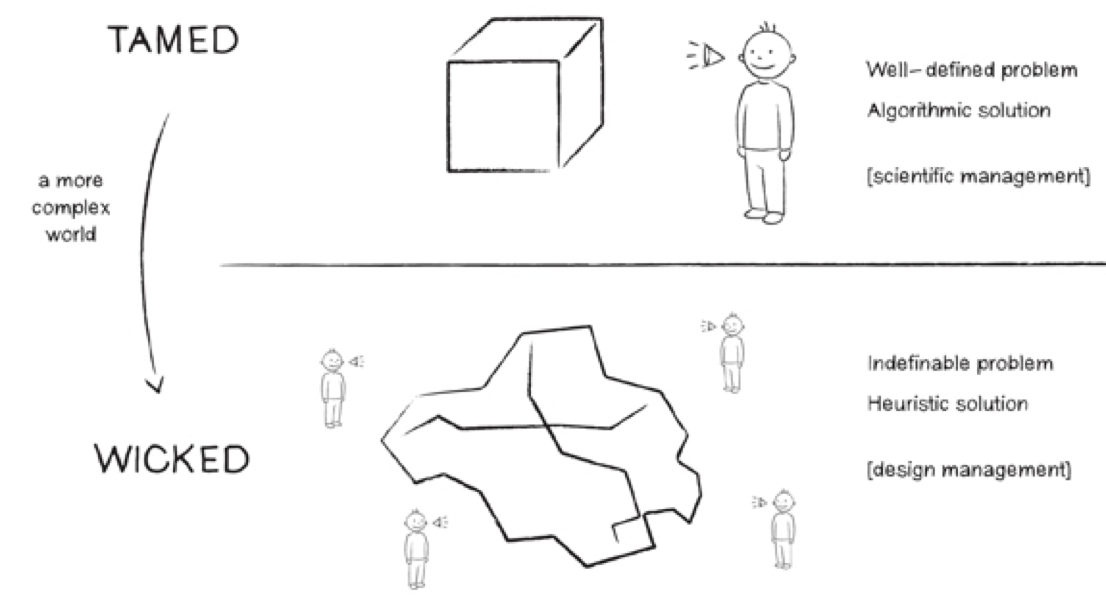
\includegraphics[width=70mm]{P2023.AIBCCSS.IlConcettoDiSoftware/pic-03.png}
\end{center}

\end{small}

\begin{center}
\tiny
\url{https://vivifychangecatalyst.wordpress.com/2015/06/28/wicked-problems-innovation-and-project-masiluleke}

\end{center}


\end{frame}

%====================================================================================

\begin{frame}{\centerline{I problemi tame}}

\begin{itemize}
\item Hanno una descrizione ben definita e stabile
\item Hanno un punto di fermata, ovvero una chiara definizione di quando la soluzione \`{e} stata trovata
\item Hanno una soluzione che pu\`{o} essere definita come giusta o sbagliata
\item Appartengono a una classe di problemi simili che possono essere tutti risolti in un modo simile
\item Hanno soluzioni che possono essere provate e abbandonate con facilit\`{a}
\item Hanno un insieme limitato di possibili soluzione
\end{itemize}
%Succi.B7 c1.2. p.9
\begin{center}
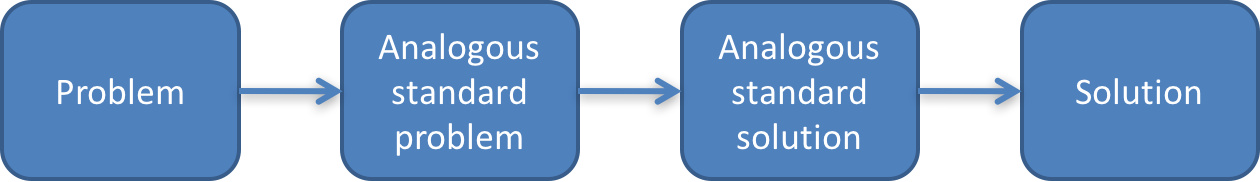
\includegraphics[width=80mm]{P2023.AIBCCSS.IlConcettoDiSoftware/pic-04.png}
\end{center}

\begin{center}
\tiny
\url{http://www.slideshare.net/curtistim/wicked-issues-taming-problems-and-systems}
\end{center}

\end{frame}

%====================================================================================

\begin{frame}{\centerline{I problemi wicked (1/4)}}

\small
\begin{itemize}
\item I problemi wicked non hanno una formulazione chiara, univoca ed analitica e definire il problema \`{e} gi\`{a} un passo verso la soluzione.

\item Un problema wicked riguarda spesso una serie di questioni con interdipendenze e vincoli che cambiano nel tempo inseriti in un contesto dinamico e in evoluzione.

\item Analogamente, ogni volta si cerca di creare una soluzione si ha una nuova e, si spera, migliore comprensione del problema, e quindi formulare il problema e risolvere il problema sono praticamente la stessa cosa.


\end{itemize}
%Succi.B7 c1.2. p.9

\end{frame}

%====================================================================================

\begin{frame}{\centerline{I problemi wicked (2/4)}}

\small
\begin{itemize}
\item Il processo di soluzione procede di solito per tentativi successivi finch\'{e} le risorse per la soluzione sono concluse, gli stakeholder hanno perso interesse in ulteriori raffinamento della soluzione proposta.

\item Le soluzioni ai problemi wicked non sono vere o false ma pi\`{u} o meno accettabili. Visto che, come detto, non c'\`{e} un criterio non ambiguo per definire il problema come \textcolor{cyan}{risolto}, pu\`{o} essere problematico convincere tutti gli stakeholder che si \`{e} raggiunta una soluzione sufficientemente buona.

\item Non c'\`{e} un test diretto o definitivo per una soluzione a un problema wicked. Soluzioni a questi problemi generano flussi di conseguenze i cui effetti finali sono imprevedibili.


\end{itemize}
%Succi.B7 c1.2. p.9

\end{frame}

\begin{frame}{\centerline{I problemi wicked (3/4)}}

\small
\begin{itemize}
\item Ogni soluzione ad un problema wicked ha conseguenze irreversibili. 
\begin{itemize}
\item Bisogna porre attenzione nel gestire presunte soluzioni: ad esempio una volta che una pubblicit\`{a} di un'offerta \`{e} rilasciata \`{e} impossibile o, quanto meno, difficoltoso, cambiare tale offerta.
\end{itemize}

\item I problemi wicked non hanno un insieme chiaro e universalmente accettato di possibili soluzioni. I vari stakeholder possono avere opinioni diverse di quelle che sono accettabili.

\item Ogni problema wicked \`{e} sostanzialmente unico e non \`{e} facile trovare problemi analogi precedentemente risolti e ben documentati in modo che le loro soluzioni possano essere replicate.

\end{itemize}
%Succi.B7 c1.2. p.9

\end{frame}

\begin{frame}{\centerline{I problemi wicked (4/4)}}

\small
\begin{itemize}

\item Il problema wicked pu\`{o} essere considerato un sintomo di un altro problema.

\item Le cause di un problema wicked possono essere spiegate in modi molto diversi.

\item Gli stakeholder hanno spesso idee diverse e pure che cambiano su che cosa sia il problema, la sua natura, le sue cause, e le soluzioni da provare.

\item Il problema wicked non pu\`{o} rimanere irrisolto ed il progetto associato non pu\`{o} fallire.
\begin{itemize}
\item Nonostante l'impossibilit\`{a} di esprimere il problema e la soluzione in modo analitico, il fallimento non \`{e} un'opzione accettabile.
\end{itemize}

\end{itemize}
%Succi.B7 c1.2. p.9

\end{frame}

\begin{frame}{\centerline{Lo sviluppo software \`{e} un problema wicked (1/2)}}

\small
\begin{itemize}
\item \`{E} molto difficile pianificare all'inizio del progetto tutto lo sviluppo futuro considerando ogni possibile eventualit\`{a}

\item Un prodotto software non \`{e} praticamente mai perfetto o finito: quando viene messo in uso subito appaiono nuovo requisiti

\item Non esiste una soluzione unica a un problema di ingegneria del software

\item Non possiamo sapere a priori il livello a cui una implementazione di un sistema soddisfa i requisiti iniziale finch´\`{e} non la implementiamo.

\item Le scelte sono alle volte molto costose da essere ribaltate. L'ultima spiaggia è buttare via il prodotto fino a quel punto sviluppato e ricominciare da capo.

\end{itemize}
%Succi.B7 c1.3. p.10

\end{frame}
\begin{frame}{\centerline{Lo sviluppo software \`{e} un problema wicked (2/2)}}

\small 
\begin{itemize}
\item Ci sono infiniti modi per risolvere un problema di sviluppo software.

\item Ogni progetto di sviluppo software \`{e} un unicum.

\item La presenza di problemi wicked si struttura a livelli multipli: le scelte dei \textcolor{red}{\textit{migliori}} database, interfacce utente, sistemi operativi, hardware sono tutti problemi wicked.

\item Il problema che lo sviluppo software deve risolvere \`{e} visto in modo diverso dai diversi stakeholder del sistema: clienti, utenti, sviluppatori, manutentori, operatori di database, ecc.

\item Lo sviluppo software in s\'{e} consuma risorse, quindi fare un errore, ovvero sviluppare qualche cosa che il cliente non vuole, non \`{e} una opzione accettabile.

\end{itemize}
%Succi.B7 c1.3. p.10

\end{frame}

%---------------------------------------------
\begin{frame}{\centerline{Come controllare il processo (1/3)}}


Michael L. Harris ha proposto un meccanismo efficace per classificare i diversi tipi di controllo e le circostanze in cui funzionano meglio.
\newline 

La selezione del meccanismo pi\`{u} efficace dipende da due fattori:
\begin{itemize}
\item  l'abilit\`{a} di misurare il risultato (output), ovvero la ``misurabilit\`{a}'' e

\item  l'abilit\`{a} di specificare in dettaglio i passi necessari per svolgere un dato compito, la ``specificabilit\`{a}''.
\end{itemize}
\end{frame}
%=============================================

%---------------------------------------------
\begin{frame}{\centerline{Come controllare il processo (2/3)}}

Mettendo questi due fattori in un diagramma bidimensionale otteniamo quattro aree::
\begin{itemize}

\item  l'area con il pi\`{u} alto livello di misurabilit\`{a} e specificabilit\`{a};

\item  l'area in cui si ha un alto livello di misurabilit\`{a} ma poca specificabilit\`{a};

\item  l'area con poca misurabilit\`{a} e con il pi\`{u} alto livello di specificabilit\`{a};

\item  l'area in cui non possiamo n\'{e} misurare con precisione il risultato n\'{e} definire con precisione i risultati del problema 

\end{itemize}
\end{frame}
%=============================================

%---------------------------------------------
\begin{frame}{\centerline{Come controllare il processo (3/3)}}


\begin{center}
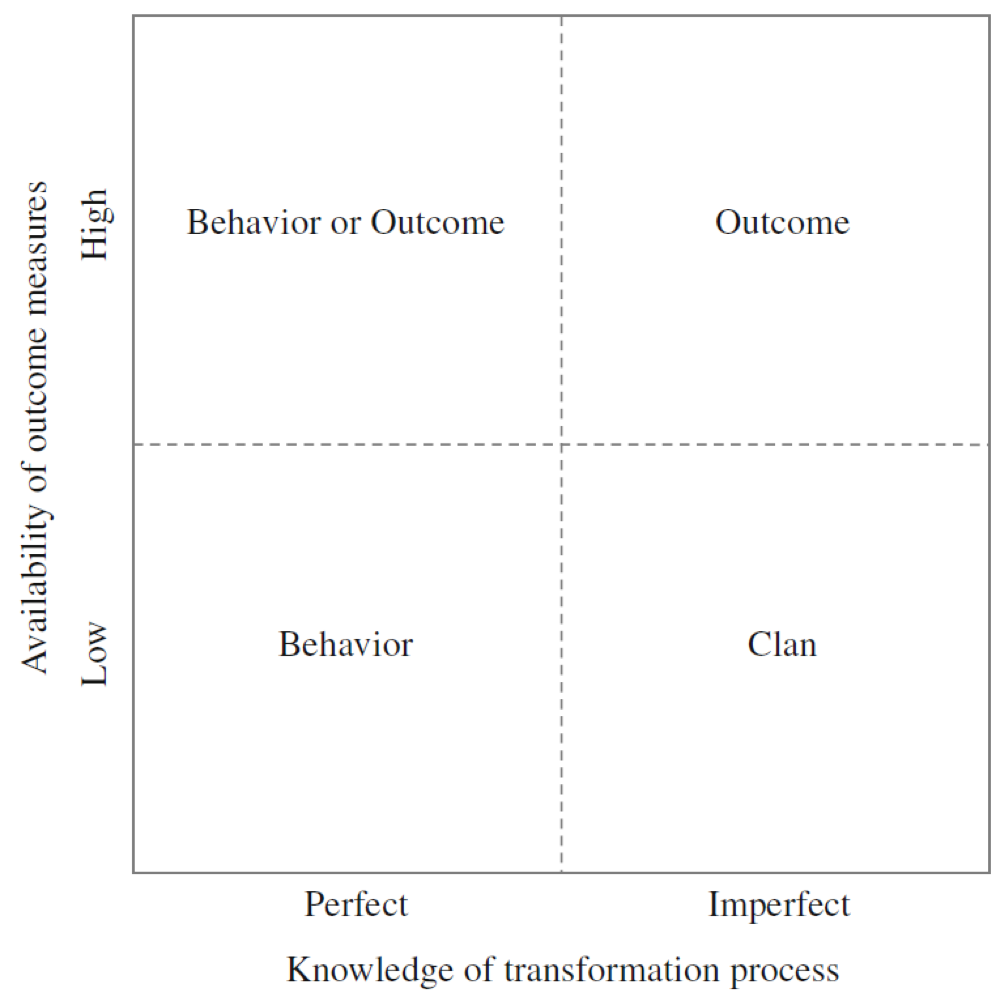
\includegraphics[width=70mm]{P2023.AIBCCSS.IlConcettoDiSoftware/img-img03.png}
\end{center}
\end{frame}
%=============================================

\begin{frame}{\centerline{Meccanismi di coordinamento}}
7
\begin{center}

\includegraphics[width=20mm]{P2023.AIBCCSS.IlConcettoDiSoftware/img-img10.png}
\end{center}

Secondo Malone e Crowston (1994) ci sono tre modi con cui le persone si coordinano:
\begin{itemize}
\item  sequenziale o individuale (sequential)
\item  tramite risorse condivise (shared resources)
\item  tramite risultato comune (common output)
\end{itemize}

\end{frame}
%=============================================

%---------------------------------------------
\begin{frame}{\centerline{Coordinamento sequenziale}}
8

\begin{center}
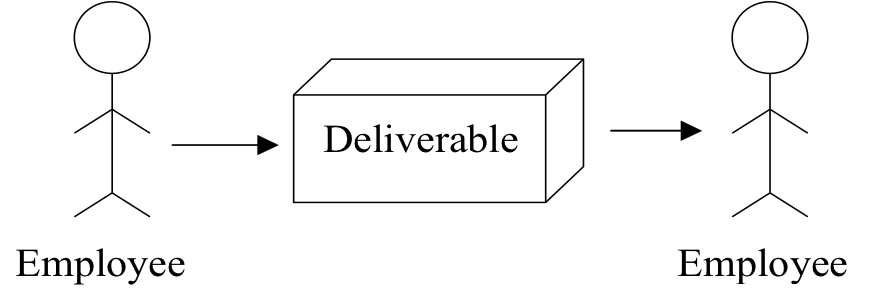
\includegraphics[width=70mm]{P2023.AIBCCSS.IlConcettoDiSoftware/img-img11.png}
\end{center}

\begin{itemize}
\item  Prima si scrive il documento di analisi


\item  Sulla base del documento di analisi si progetta il sistema


 
\end{itemize}

\end{frame}
%=============================================

%---------------------------------------------
\begin{frame}{\centerline{Coordinamento a risorse condivise}}
9
\begin{center}
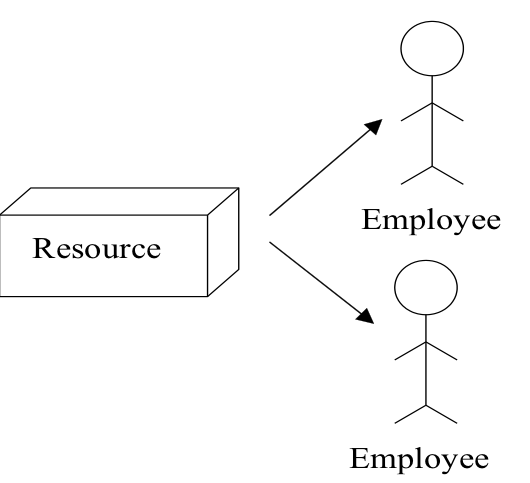
\includegraphics[width=50mm]{P2023.AIBCCSS.IlConcettoDiSoftware/img-img12.png}
\end{center}

\begin{itemize}
\item  Lo sviluppo pu\`{o} iniziare quanto il cliente ha dato il via al progetto

\item Le parti da sviluppare possono essere assegnate agli sviluppatori con un meccanismo a coda (first come, first served)


\end{itemize}


\end{frame}
%=============================================

%---------------------------------------------
\begin{frame}{\centerline{Coordinamento a risultato comune}}
0
\begin{center}
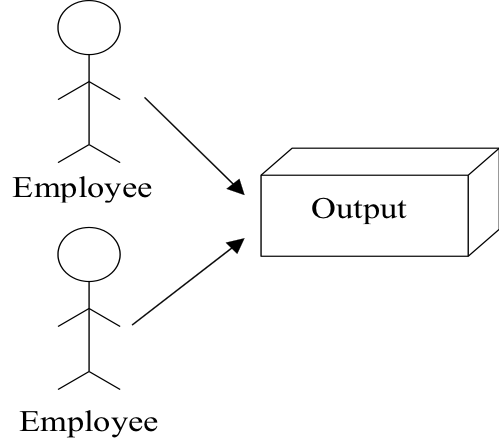
\includegraphics[width=50mm]{P2023.AIBCCSS.IlConcettoDiSoftware/img-img13.png}
\end{center}

\begin{itemize}
\item  Il responsabile del team propone un piano di lavoro per la settimane e tale piano viene approvato se il team unanimamente lo accetta

\item Il team si siede insieme e produce la versione finale che richiede l'approvazione di tutti

  
\end{itemize}


\end{frame}
%=============================================

%---------------------------------------------
\begin{frame}{\centerline{Qual \`{e} il pi\`{u} difficile?}}
1
\begin{itemize}

\item  Il pi\`{u} facile: quello sequenziale!
\item  Poi: risorse condivise -- occorre saper rispettare le priorit\`{a} di sviluppo
\item  Il pi\`{u} difficile: risultato condiviso
\begin{itemize}

\item  le persone devono lavorare insieme, mano nella mano, producendo lo stesso bene
\end{itemize}

\item La gran parte dei modelli tradizionali di sviluppo software si basano su coordinamento sequenziale

\end{itemize}

\end{frame}
%=============================================


\begin{frame}{\centerline{I modelli di sviluppo software}}

\begin{itemize}
\item Ora analizziamo brevemente i modelli di sviluppo software che sono stati proposti negli anni
\item Cerchiamo di comprendere i meccanismi di controllo e coordinamento in essere per determinare:
\begin{itemize}
\item la loro efficacia
\item la loro difficolt\`{a} di realizzazione 
\end{itemize}
\end{itemize}
\end{frame}


\begin{frame}{\centerline{Il modello di sviluppo a cascata}}


\begin{itemize}
    \item Il modello di sviluppo \textcolor{red}{a cascata} \`{e} stato il primo modo con cui si \`{e} tentato di riuscire a creare un \textcolor{red}{prodotto software che risponda ai requisiti}.
    \item Per ottenere tale risultato, si sono definiti passi precisi che rispecchiano il mondo manufatturiero in cui, ad esempio, la progettazione avviene dopo l'analisi, lo sviluppo dopo la pregettazione, e la verifica di correttezza dopo lo sviluppo.
\item Il tutto sembra molto logico ...
\end{itemize}


\end{frame}

\begin{frame}{\centerline{Il modello di sviluppo a cascata -- schema}}


\begin{center}
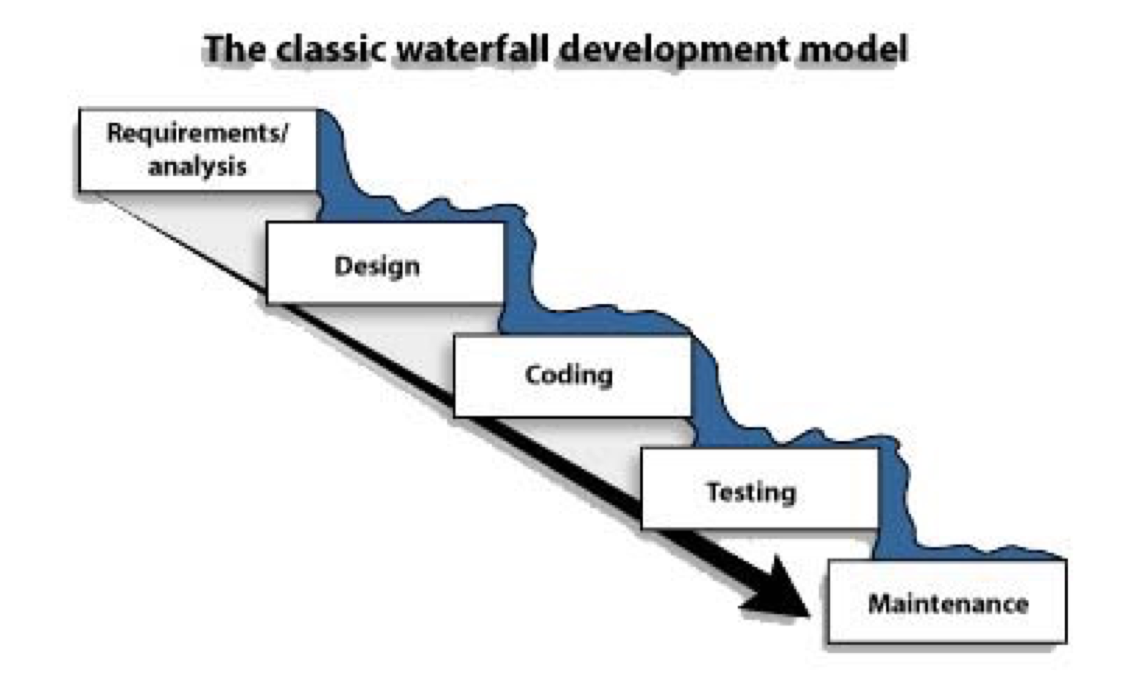
\includegraphics[width=80mm]{P2023.AIBCCSS.IlConcettoDiSoftware/img-02.png}
\end{center}
\vspace{0.5cm}

\begin{center}
\tiny
Fonte: \url{http://www.railshorde.com/blog/waterfall-development-model}

\end{center}
\end{frame}

\begin{frame}{\centerline{Il modello di sviluppo a cascata -- fasi (1/3)}}


\textcolor{red}{\bf Pianificazione e Requisiti:} Tutti i possibili requisiti del sistema da sviluppare sono raccolti e viene sviluppato un piano per lo sviluppo affinch\'{e} tutto sia fatto nei tempi e nei costi prestabiliti.
\newline

\textcolor{red}{\bf Analisi e Progettazione del sistema:} I requisiti precedentemente elicitati sono messi in forma scritta, analizzati con cura e quindi viene sviluppato un progetto (design) del sistema. Questo progetto rappresenta il riferimento del software da sviluppare. Il progetto di sistema serve a definire i bisogni di hardware e di software e specifica anche l'architettura di massima.
\newline

\begin{center}
\tiny
Fonte: \url{http://www.railshorde.com/blog/waterfall-development-model}
\end{center}

\end{frame}

\begin{frame}{\centerline{Il modello di sviluppo a cascata -- fasi (2/3)}}

\textcolor{red}{\bf Costruizione:} Con le informazioni raccolte nei documenti di progetto incomincia la codifica. Gli sviluppatori sono responsabili per il codice prodotto. Di solti si parte focalizzandosi su piccole unit\`{a} e poi il sistema cresce componendo tali piccole unit\`{a} in entit\`{a} pi\`{u} ``grandi'' per la successiva integrazione. Si noti che il concetto di grande \`{e} molto soggettivo.
\newline

\textcolor{red}{\bf Test di unit\`{a}, integrazione e test finale di sistema:} Tutte le unit\`{a} sviluppate singolarmente nella fase di costruzione sono verificate (testate) singolarmente, e quindi integrate nel prodotto finale. Il prodotto finale completo \`{e} quindi testato complessivamente per rilevare ulteriori errori, difetti, non conformit\`{a} con i desideri dei clienti.
\newline

\begin{center}
\tiny
Fonte: \url{http://www.railshorde.com/blog/waterfall-development-model}
\end{center}


\end{frame}

\begin{frame}{\centerline{Il modello di sviluppo a cascata -- fasi (3/3)}}



\textcolor{red}{\bf Consegna del sistema:} Dopo che ci si \`{e} assicurati della qualit\`{a} del prodotto con il test, il prodotto viene consegnato al cliente.
\newline

\textcolor{red}{\bf Manutenzione:} Per gestire tutte le problematiche che avvengono dopo la consegna del prodotto, una specifica fase di manutenzione viene prevista. Inoltre, data la costante evoluzione dei sistemi hardware e software la fase di manutenzione si occupa dell'aggiornamento del sistema in modo che il cliente abbia sempre un sistema aggiornato ed efficace.

\newline

\begin{center}
\tiny
Fonte: \url{http://www.railshorde.com/blog/waterfall-development-model}
\end{center}

\end{frame}

\begin{frame}{\centerline{Il modello di sviluppo a cascata -- commento}}

\textcolor{blue}{\bf Ovviamente tutto quanto detto sopra \`{e} lo sviluppo a cascata nei desideri di chi lo ha ideato ... una sorta di lettera a babbo natale!}

\begin{center}

\includegraphics[width=30mm]{P2023.AIBCCSS.IlConcettoDiSoftware/san_nicolo-201x300.jpg}
\end{center}
\vspace{0.5cm}

\begin{center}
\tiny
Fonte: \url{https://www.triesteallnews.it/wp-content/images/2019/12/san_nicolo-201x300.jpg}
\end{center}


\end{frame}


\begin{frame}{\centerline{Vantaggi del modello di sviluppo a cascata}}


\begin{itemize}
\item  Semplice da usare e capire.

\item  Ogni fase viene sviluppata individualmente in modo che ci si dedica a fondo e con concentrazione ad una azione alla volta.

\item  Funziona bene per piccoli progetti dove i requisiti sono ben compresi.

\item  Ogni fase ha le attivit\`{a} che deve svolgere in modo preciso.

\item  Ogni fase \`{e} documentata nel dettaglio per evitare qualunque possibile ambiguit\`{a}.

\item \textcolor{red}{Notate di nuovo che questi sono i desiderata \ldots{} che poi la realt\`{a} corrisponda ad essi, \`{e} un altro discorso.}

\end{itemize}

\end{frame}
\begin{frame}{\centerline{Svantaggi del modello di sviluppo a cascata}}


\begin{itemize}
\item Il primo svantaggio che appare \`{e} che il tutto \`{e} molto sequenziale e si pu\`{o} fare solo una cosa alla volta; \textcolor{red}{questo confligge con la natura combinatoria e iterativa dei problemi wicked.} 

\item  I requisiti devono essere definiti all'inizio; se un requisito viene identificato dopo, esso non pu\`{o} essere inserito con facilit\`{a} nel processo di sviluppo.


\item Il modello a cascata non permette facilmente iterazioni e il progetto nella sua interezza va integrato alla fine.

\item I clienti possono avere accesso al progetto solo alla fine. Non sono rilasciati prototipi o sistemi parziali in anticipo.
\end{itemize}

\end{frame}

\begin{frame}{\centerline{Applicabilit\`{a} del modello di sviluppo a cascata}}


\begin{itemize}

\item  Non ci devono essere requisiti ambigui.

\item  I requisiti devono essere ben documentati e fissati in anticipo.

\item  La tecnologia in uso (hardware, sistema operativo, API, ...) non deve cambiare durante il progetto.

\item  La definizione del prodotto deve essere stabile.

\item  Risorse con esperienza devono essere presenti per aiutare lo sviluppo del prodotto.
\end{itemize}

\end{frame}

\begin{frame}{\centerline{Evoluzioni e raffinamenti}}


\begin{itemize}

\item  Il modello di sviluppo a V, con gli associati
\begin{itemize}
\item modello a dente di sega e 
\item modello a dente di squalo
\end{itemize}

\item  Lo sviluppo incrementale.

\item  Il modello prototipale.

\end{itemize}

\end{frame}


\begin{frame}{\centerline{Modello di sviluppo a spirale}}

\begin{center}
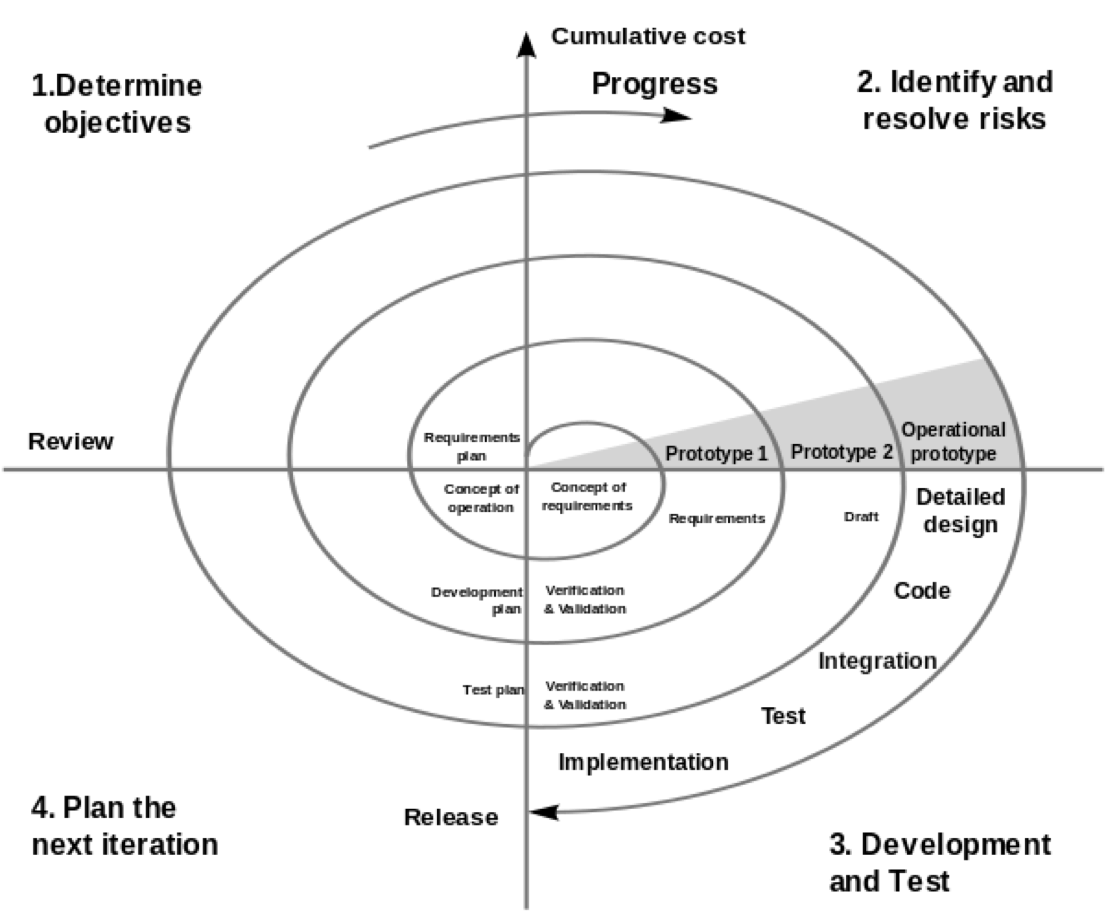
\includegraphics[width=80mm]{P2023.AIBCCSS.IlConcettoDiSoftware/img-03.png}
\end{center}

\begin{center}
\tiny
Fonte: \url{https://en.wikipedia.org/wiki/Spiral\_model}
\end{center}

\end{frame}

\begin{frame}{\centerline{Principi del modello di sviluppo a spirale}}


Il modello di sviluppo a spirale \est{} un approccio iterativo allo sviluppo software in cui ogni ciclo della spirale ha le seguenti caratteristiche:

\begin{itemize}

\item  Determinazione degli artifatti da sviluppare concorrente e non sequenziale

\item  Inclusione in ogni ciclo della spirale dei sequenti elementi:

\begin{itemize}
\item  revisione degli obiettivi e dei vincoli degli stakeholder critici del sistema,
\item  analisi di processi e prodotti alternativi,
\item  identificazione e risoluzione dei rischi,
\item  revisione con gli stakeholder,
\item  esplicita decisione di continuare o terminazione del progetto.
\end{itemize}
\end{itemize}
\end{frame}
\begin{frame}{\centerline{Ingredienti del modello di sviluppo a spirale}}


\begin{itemize}
\item  Uso dell'analisi del rischio per determinare il livello di sforzo necessario ad ogni attivit\`{a} all'interno di ogni ciclo della spirale

\item  Gestione all'interno di ogni ciclo della spirale degli accordi con gli stakeholder sulla struttura e sul contenuto del processo di sviluppo.

\item  Enfasi su attivit\`{a} e artefatti del sistema e del processo di produzione nel loro insieme e non soltanto sul software risultante alla fine.

\end{itemize}


\end{frame}

%---------------------------------------------
\begin{frame}{\centerline{L'\textcolor{red}{Agile Manifesto} (1/2)}}
\begin{itemize}
    \item Nel Febbraio 2001 un gruppo di softwaristi molto esperti formalizz\`{o} un nuovo modo di sviluppare software in un \textcolor{red}{Manifesto}
    \item Questo manifesto sintetizzava pratiche che si erano sviluppate nel tempo, alcune che risalivano agli albori dello svilupo software
    \item Di fatto il manifesto era una istanziazione del modello di sviluppo a spirale
    \item Al manifesto faceva poi seguito una lista di principi
\end{itemize}
\end{frame}


%---------------------------------------------
\begin{frame}{\centerline{L'\textcolor{red}{Agile Manifesto}(2/2)}}

\begin{center}
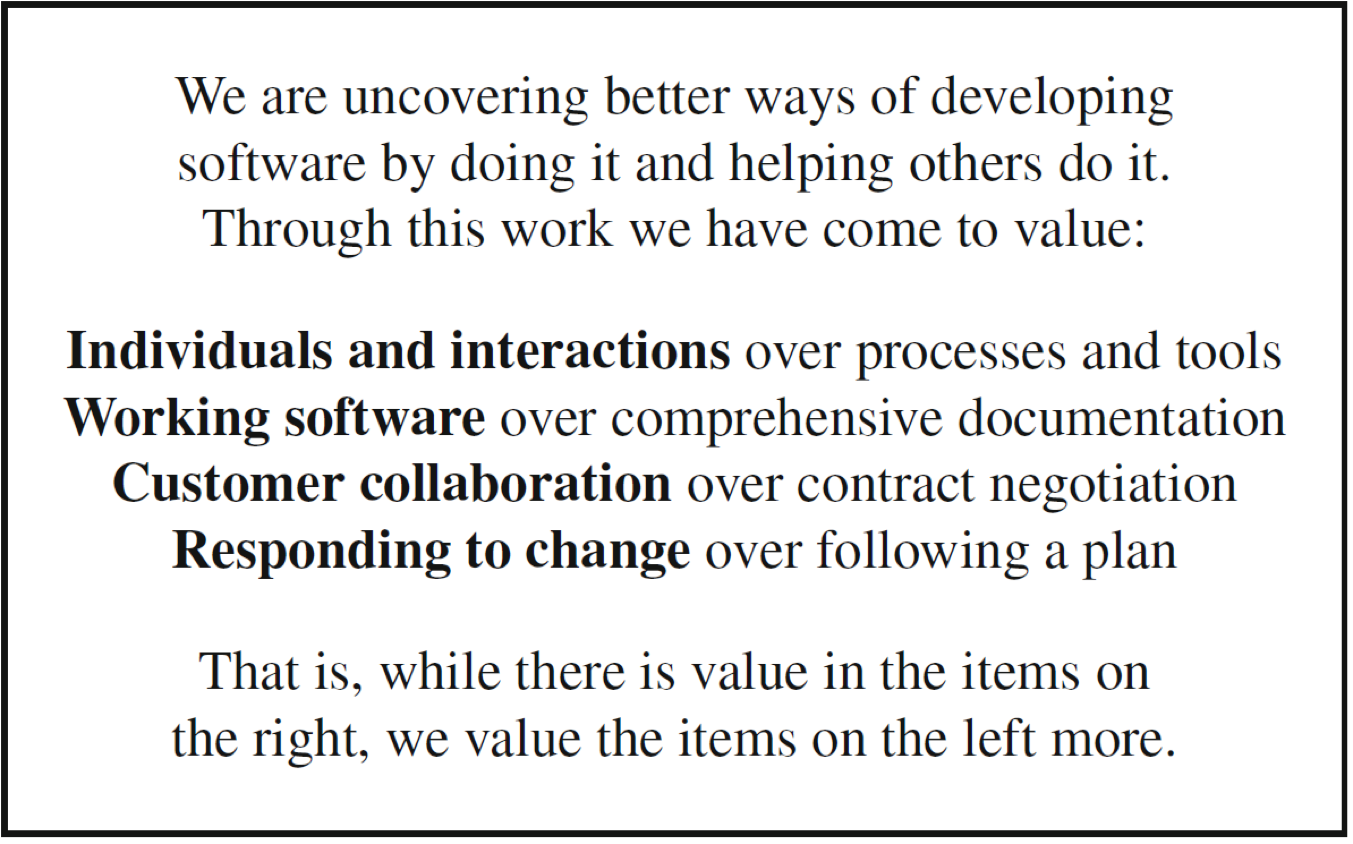
\includegraphics[width=80mm]{P2023.AIBCCSS.IlConcettoDiSoftware/img-img00.png}
\end{center}
\begin{center}
\tiny
Fonte: \url{https://agilemanifesto.org}
\end{center}

\end{frame}
%=============================================


%---------------------------------------------
\begin{frame}{\centerline{Agile Manifesto}}


L'``Agile Manifesto'' identifica due insiemi di valori:
\begin{itemize}
    \item quelli a destra del documento
    \item quelli a sinistra del documento
\end{itemize}

\begin{center}
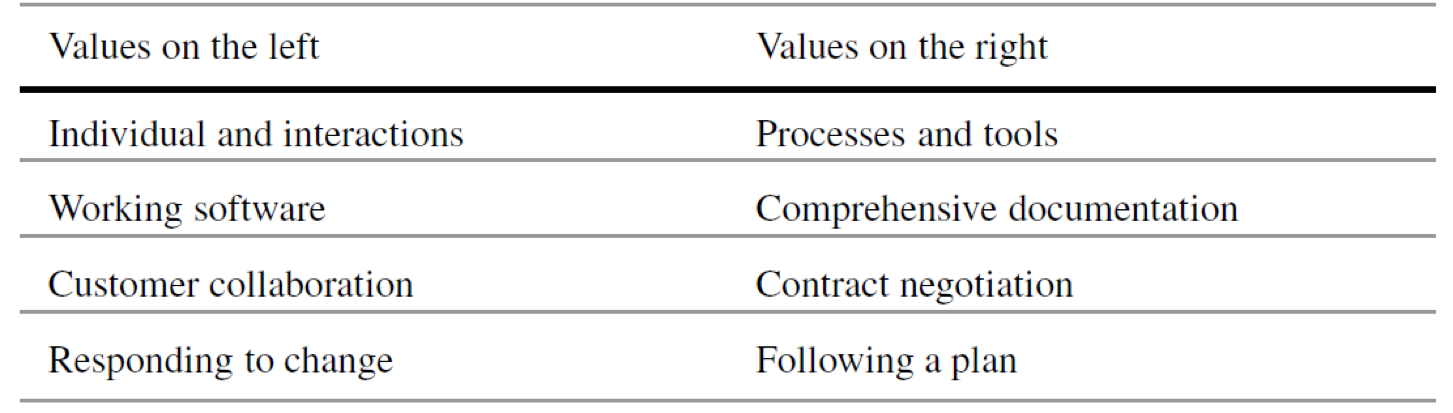
\includegraphics[width=120mm]{P2023.AIBCCSS.IlConcettoDiSoftware/img-img01.png}
\end{center}
\end{frame}
%=============================================

%---------------------------------------------
\begin{frame}{\centerline{Principi dell'Agile Manifesto (1/2)}}

\begin{itemize}
\item  Our highest priority is to satisfy the customer through early and continuous delivery of valuable software
\item  Welcome changing requirements, even late in development, Agile processes harness change for the customer's advantage
\item  Business people and developers must work together daily throughout the project
\item  Deliver working software frequently, from a couple of weeks to a couple of months, with a preference to the shorter timescale
\item  Build projects around motivated individuals
\item  Give them the environment and support they need, and trust them to get the job done
\item  The most efficient and effective method of conveying information to and within a development team is face-to-face conversation
\end{itemize}

\begin{center}
\tiny
Fonte: \url{https://http://agilemanifesto.org/principles.html}
\end{center}

\end{frame}
%=============================================

%---------------------------------------------
\begin{frame}{\centerline{Principi dell'Agile Manifesto (2/2)}}

\begin{itemize}
\item  Working software is the primary measure of progress
\item  Agile processes promote sustainable development. The sponsors, developers, and users should be able to maintain a constant pace indefinitely
\item  Continuous attention to technical excellence and good design enhances agility
\item  Simplicity -- the art of maximizing the amount of work not done -- is essential
\item  The best architectures, requirements, and designs emerge from self-organizing teams
\item  At regular intervals, the team reflects on how to become more effective, then tunes and adjusts its behavior accordingly
\end{itemize}

\begin{center}
\tiny
Fonte: \url{https://http://agilemanifesto.org/principles.html}
\end{center}

\end{frame}
%=============================================


%=============================================



\begin{frame}
{\centerline{Domande?}}
\vspace{1cm}
\begin{center}
    \LARGE{Fine delle prime tre lezioni.}
\end{center}

\end{frame}


\end{document}
